\documentclass[a4paper,12pt, final]{report}
\usepackage[utf8]{inputenc}
\usepackage[T1]{fontenc}
\usepackage[english]{babel}

\usepackage[table]{xcolor}

% ===========================
% === PACKAGES DE BASE ===
% ===========================
\usepackage{subfig}
\usepackage{newtxtext,newtxmath}  % Police Times New Roman améliorée
\usepackage{microtype}
\usepackage[top=2cm, bottom=2cm, left=2.5cm, right=2.5cm]{geometry}
\usepackage{parskip}
\setlength{\parskip}{0.5\baselineskip}
\usepackage{indentfirst}
\usepackage{hyperref}
\usepackage{fancyhdr}
\setlength{\headheight}{14.5pt}
\addtolength{\topmargin}{-2.5pt}
\usepackage[nottoc]{tocbibind}
\usepackage{underscore}
\usepackage{setspace}
\onehalfspacing  % Interligne 1.5
\usepackage{tabularx}

% ===========================
% === PACKAGES MATH ===
% ===========================
\usepackage{amsmath}
\usepackage{amssymb}
\usepackage{amsfonts}
\usepackage{mathrsfs}
\usepackage{siunitx}

% ===========================
% === GRAPHIQUES & TABLEAUX ===
% ===========================
\usepackage{graphicx}
\usepackage{float}
\usepackage[font=normalsize]{caption}  % Légendes lisibles
\usepackage{booktabs}
\usepackage{array}
\usepackage{longtable}
\usepackage{makecell}
\usepackage{soul}

% ===========================
% === ALGORITHMES & CODE ===
% ===========================
\usepackage{algorithm}
\usepackage{algorithmic}
\usepackage{listings}

% ===========================
% === AUTRES PACKAGES ===
% ===========================
\usepackage{acronym}
\usepackage{enumitem}
\usepackage{dirtytalk}
\usepackage{textpos}
\usepackage{tikz}
\usepackage{titlesec}
\usepackage{url}
\usepackage{pdfpages}

% ===========================
% === CONFIGURATION TITRES ===
% ===========================
\titleformat{\chapter}[block]
{\normalfont\Large\bfseries}{\thechapter}{1em}{}
\titlespacing*{\chapter}{0pt}{24pt}{12pt}

\titleformat{\section}[block]
{\normalfont\large\bfseries}{\thesection}{1em}{}
\titlespacing*{\section}{0pt}{24pt}{12pt}

\titleformat{\subsection}[block]
{\normalfont\normalsize\bfseries}{\thesubsection}{1em}{}
\titlespacing*{\subsection}{0pt}{12pt}{6pt}

\titleformat{\subsubsection}[block]
{\normalfont\normalsize\bfseries}{\thesubsubsection}{1em}{}
\titlespacing*{\subsubsection}{0pt}{12pt}{6pt}

% ===========================
% === EN-TÊTES & PIEDS DE PAGE ===
% ===========================
\pagestyle{fancy}
\fancyhf{}
\fancyhead[L]{\footnotesize\leftmark}
\fancyhead[R]{\footnotesize\thepage}
\renewcommand{\headrulewidth}{0pt}

% ===========================
% === BIBLIOGRAPHIE ===
% ===========================
\usepackage[sort&compress,numbers]{natbib}

% ===========================
% === HYPERLIENS ===
% ===========================
\hypersetup{
    colorlinks=true,
    linkcolor=black,
    urlcolor=blue,
    citecolor=black,
    pdftitle={},
    pdfauthor={},
    pdfsubject={}
}

% ===========================
% === DÉBUT DU DOCUMENT ===
% ===========================
\begin{document}

% pagePFE.tex — English Title Page with Jury Table at Bottom
\begin{titlepage}
\pagestyle{empty}

% Full-page background using TikZ
\begin{tikzpicture}[remember picture, overlay]
  % Background image
  \node[inner sep=0pt] at (current page.center) {
    
\includegraphics[width=\paperwidth, height=\paperheight]{images/bg-wave.png}
  };

  % Logos
  \node[anchor=north west, xshift=1.5cm, yshift=-1.5cm] at (current page.north west) {
    
\includegraphics[height=2cm]{images/UM_logo.png}
  };
  
  \node[anchor=north east, xshift=-1.5cm, yshift=-1.5cm] at (current page.north east) {
    
\includegraphics[height=2cm]{images/ISIM_logo.png}
  };
\end{tikzpicture}

\begin{center}
    {Republic of Tunisia\\
    ***** \\
    Ministry of Higher Education and Scientific Research\\
    ***** \\[0.2cm] \textbf{Higher Institute of Computer Science and Mathematics of Monastir\\}
    ***** \\[0.2cm]
    Computer Science Department}\\[1cm]
    \vspace{0.6cm}

    \Large\textbf{End of Studies Project Thesis} \\
    \vspace{0.4cm}

    Presented to obtain: \\
    \textbf{National Professional Master’s Degree in Computer Science} \\
    \vspace{0.3cm}
    Speciality: \\
    \textbf{Data Science}


    % Title
    \rule{\linewidth}{0.5mm} \\[0.1cm]
    {\large \bfseries Development of a Recommendation System \\and AI Assistant for a Nutritional Application
    \\[0.1cm] }
    \rule{\linewidth}{0.5mm} \\[0.5cm]

    \vspace{1cm}
    \large Submitted by: \\
    \textbf{Belgacem CHAIBI} \\

    \vspace{0.6cm}

    Host Company: \\
    \textbf{ONERTECH} \\
    \vspace{0.6cm}

    Defended on  01/10/2025 \\

    \vspace{0.1cm}
    Defended on 01/10/2025 before the committee composed of:
    \end{center}
    \begin{tabular}{ p{5cm} p{3cm} p{5cm}}
      M./Mme  ........... & & President \\
      M./Mme  ............ & & Reporter \\
      Mme Asma KERKENI  & & Academic Supervisor \\
      M. Marwen RHAYEM & & Professional Supervisor \\
    \end{tabular}

    \vspace{0.3cm}
    \centering
    \textbf{Academic Year: 2024--2025}


\end{titlepage}


\chapter*{Signatures}
\thispagestyle{empty}
\bigskip
\begin{center}
\ {Host Company Supervisor: Mr.Marwen RHYEM LastName}
\bigskip

\includegraphics[width=0.8\textwidth]{images/sig.png}
\end{center}

\bigskip
\begin{center}
\ {ISIMM Supervisor: Mrs. }
\bigskip

\includegraphics[width=0.8\textwidth]{images/sig.png}
\end{center}
\newpage
\section*{Dedication}

\vspace{1cm}
This work is dedicated with profound love and gratitude to those who have been the pillars of my strength and the source of my inspiration.
\medskip

To my father, \textbf{Sadek CHAIBI}, whose unwavering belief in me has been my greatest source of motivation. Your daily encouragement, your tireless efforts, and your constant support have shaped me into who I am today.  All of my achievements are a reflection of your guidance and love.
\medskip

To my beloved mother, \textbf{Arroussia Abed}, whose boundless love and sacrifices have been my foundation. Through countless sleepless nights when I was unwell, through every moment of care and tenderness, you have shown me the true meaning of unconditional love. I cherish every small gesture, every word of comfort, and every moment of support you have given me. This success is my gift to you, a token of my endless appreciation and love.
\medskip

To my brother \textbf{Montasser CHAIBI}, who fill my days with hope, love, and inspiration. Your presence in my life is a constant reminder of what truly matters, and your influence motivates me to strive for excellence every single day.
\medskip

To my dear sisters, \textbf{Nesrine CHAIBI}, \textbf{Soumaya CHAIBI} and \textbf{Sirine CHAIBI}, whose extraordinary support during the previous years have given me the confidence to pursue my dreams. Your belief in me has been a source of strength that I can not put into words.
\medskip

To all my family members, whose collective support has been the wind beneath my wings.
\medskip

To my dear friends, who have stood by me at every step of this journey, offering encouragement, sharing in my struggles, and celebrating my victories as their own.
\medskip

This achievement belongs to all of you, for it is through your love, support, and belief that I have reached this milestone.
\newpage
\chapter*{Acknowledgments}
\addcontentsline{toc}{chapter}{Acknowledgments}

I would like to express my sincere gratitude to all those who contributed to the successful completion of this project.

First and foremost, I extend my deepest appreciation to my academic supervisor, \textbf{Mm. Asma KERKENI}, for her unwavering support, invaluable guidance, and constant encouragement throughout this internship. Her expertise and mentorship have been instrumental in shaping both this work and my professional development.

I am equally grateful to the esteemed members of the evaluation committee: Mr. \textbf{******}, the committee president, and \textbf{******}, the report examiner, for their time, consideration, and valuable insights in reviewing this work.

My heartfelt thanks go to my professional supervisor, \textbf{Mr. Marwen RHYEM}, whose practical guidance and industry expertise provided me with invaluable real-world perspective and helped bridge the gap between academic theory and professional practice.

I would also like to acknowledge the entire team at ONRTECH for creating such a welcoming and collaborative environment. Their willingness to share knowledge, provide feedback, and include me as part of the team made this experience both enriching and memorable.

I extend my gratitude to all my professors and the entire academic community at the Higher Institute of Computer Science and Mathematics of Monastir (ISIMM) for their dedication to excellence in education. Their commitment to fostering knowledge and developing our skills has been fundamental to my academic growth and has prepared me for the challenges of this project.

Finally, I am deeply grateful to everyone who has supported me throughout this academic journey. Your encouragement, patience, and belief in my abilities have been the foundation of my success. This achievement would not have been possible without each of you, and I am truly thankful for your contributions to my growth and learning.

\chapter*{Abstract}

This graduation project, carried out at ONRTECH between February and August 2025, is part of our final year of the Professional Master’s degree in Data Science at the Higher Institute of Computer Science and Mathematics of Monastir (ISIMM). It focuses on the development of \textit{VitamiNurse}, an innovative application designed to help users make informed and personalized food choices. Based on artificial intelligence, it evaluates products, suggests healthier alternatives, and delivers real-time interactive support.

Developed using Scrumban and CRISP-DM methodologies, the VitamiNurse project is structured around several components, including a data pipeline, a hybrid recommendation system, and an intelligent chatbot. Together, these elements create a dynamic and user-friendly tool enabling users to make healthier and more balanced food choices.

\noindent\textbf{Keywords:} ETL, Recommendation Systems (RS), Machine Learning, Generative AI, Chatbot, ANN, SentenceTransformers.

\newpage
\chapter*{Résumé}
Ce projet de fin d’études, réalisé à l’ONRTECH entre février et août 2025, s’inscrit dans le cadre de notre dernière année de Master Professionnel en Science des Données à l’Institut Supérieur d’Informatique et de Mathématiques de Monastir (ISIMM). Il porte sur le développement de \textit{VitamiNurse}, une application innovante conçue pour aider les utilisateurs à faire des choix alimentaires éclairés et personnalisés. Basée sur l’intelligence artificielle, elle évalue les produits, suggère des alternatives plus saines et offre un accompagnement interactif en temps réel.

Développé à l’aide des méthodologies Scrumban et CRISP-DM, le projet VitamiNurse s’articule autour de plusieurs composants, dont un pipeline ETL, un système de recommandation hybride et un chatbot intelligent. Ensemble, ces éléments créent un outil dynamique et convivial permettant aux utilisateurs de faire des choix alimentaires plus sains et plus équilibrés.

\noindent\textbf{Mots-clés:} ETL, Systèmes de recommandation (SR), Apprentissage automatique, IA générative, chatbot, ANN et SentenceTransformers.

\thispagestyle{empty}
\newpage

% Table des matières
\tableofcontents
\thispagestyle{empty}

% Listes des figures et tableaux
\listoffigures
\listoftables
\thispagestyle{empty}
\newpage

% Acronymes (si besoin)
% \chapter*{List of Acronyms}
%%%%%% NB. Please ensure that the acronym list is maintained in alphabetical order.

\vspace{1cm}
\begin{itemize}
    \item \textbf{AI:} Artificial Intelligence.
    \item \textbf{ML:} Machine Learning.
    \item \textbf{ETL:}  Extract, Transform, Load.
    \item \textbf{ANN:} Approximate Nearest Neighbors.
    \item \textbf{HNSW:} Hierarchical Navigable Small World.
    \item \textbf{CRISP-DM:} Cross-Industry Standard Process for Data Mining.
    \item \textbf{NLP:} Natural Language Processing.
    \item \textbf{BERT:} Bidirectional Encoder Representations from Transformers.
    \item \textbf{LLM:} Large Language Model.
    \item \textbf{RS:} recommendation system.
    \item \textbf{KNN:} K-Nearest Neighbors.
    \item \textbf{LSTM:} Long Short-Term Memory.
    \item \textbf{LightFM:} Light Factorization Machine.
    \item \textbf{SVD:} Singular Value Decomposition.
    \item \textbf{JSON:}  JavaScript Object Notation.
\end{itemize}


%%%%%%%%%%%%%%%%%%%%%%%%%%%%%%%%%%%%%%%%%%%%%%%%
%%%%%%%%%%%%%%%%%%%%%%%%%%%%%%%%%%%%%%%%%%%%%%%%

% Corps du document
\pagestyle{fancy}
\pagenumbering{arabic}

\chapter*{General introduction}
 The rapid technological development has brought an excessive amount of data throughout entertainment sectors, fashion industries and social media platforms. People are facing a growing problem of information overload because of the excessive amount of data they receive. With endless choices at their fingertips, individuals find it increasingly difficult to sift through options and make informed decisions. In this context, recommendation systems and AI assistants have emerged as essential tools in filtering massive data and delivering personalized suggestions. With a growing societal focus on health and wellness, these technologies have become increasingly relevant for the nutrition domain. By providing scientifically grounded guidance, it address conflicting dietary information and supports healthier lifestyle choices.\\


\par From this perspective, The company ONRTECH is currently working on a major project called Vitamiurse, which aims to provide a mobile application capable of delivering personalized recommendations based on users' dietary preferences.

Within this framework, our contribution focused on developing the components related to the recommendation system and the intelligent assistant.

This report presents a comprehensive documentation of the work carried out
during my internship. It consists of four separate chapters, each addressing distinct aspects of my project. The first chapter introduces the general context of the project, presents the host company and outlines the objectives of the internship. It also describes the methodology adopted and the project architecture.\\
The second chapter focuses on the design and implementation of the data pipeline using an advanced ETL framework. The third chapter describes the development of a hybrid recommendation system. This hybrid system combines collaborative
filtering, content-based approaches, and real-time analytics. The last chapter presents the design and integration of the intelligent conversational assistant. This chapter highlights its core functionalities, its interaction with users, and its role in providing personalized nutritional guidance.

In conclusion, we mention the various strengths of this project and summarize all the work accomplished while proposing some perspectives that could further improve our solution.


\chapter{Project Context}
\section*{Introduction}
\addcontentsline{toc}{section}{Introduction}
This chapter provides an overview of the project by presenting its background and context. It begins by introducing the host company ONRTECH, followed by a detailed explanation of the
problems in the first version of VitamiNurse application. The chapter also compares existing nutrition applications to show their limitations. Next, we present our proposed solution to enhance our mobile application with advanced features such as a personalized recommendation system and an AI assistant.
The chapter concludes by establishing the methodological frameworks that will guide the management and technical execution of the project.

\section{Presentation of the host company}
\par ONRTECH\footnote{\url{https://onrtech.fr/}} is a French company, operating since 2020 and located in
Villiers-sur-Marne, France, that focuses on software development, IT consulting, and artificial intelligence.
It operates within the wider field of programming, advisory, and other digital services, delivering modern, innovative solutions tailored to evolving business needs. 
\par Since its creation, ONRTECH has rapidly grown into a trusted provider of digital services, having collaborated with numerous
clients throughout France and Europe. More than just a tech provider, it positions itself as a durable digital partner by focusing on customer satisfaction and offering customized solutions.
\begin{figure}[H]
    \centering
    
\includegraphics[width=0.25\textwidth]{images/ONRTECH_logo.jpeg}
    \caption{ONRTECH company logo}
    \label{fig:ONRTECH_logo}
\end{figure}


\newpage
\section{Internship context and project objectives}
As part of our training at the Higher Institute of Computer Science and Mathematics in Monastir, we had the opportunity to complete our end-of-studies internship at ONRTECH.

 The goal of this internship is to develop a personalized recommendation system and an AI assistant for the nutritional mobile application Vitaminurse. 
 The system presents product details, assesses the scanned product with AI, and then shows a clear conclusion of the analysis on whether the product is suitable for the user’s nutritional profile. 
 If it is not suitable, the recommendation system suggests more adapted alternatives.

In addition, it engages users in friendly conversation and provides personalized nutritional advice. By understanding the preferences, health goals, and nutritional needs of each person, Vitaminurse provides personalized advice and recommendations that actually make sense for their lifestyle and health needs. 
\subsection{First version of VitamiNurse}
The initial version of VitamiNurse exists as a simple mobile application developed by ORTECH  to enable users scan product barcodes for viewing nutritional data. The application operates in a market which presents major obstacles to its success because of intense competition. The food tracking market already has two established apps Yuka and OpenFoodFacts which makes it difficult for VitamiNurse to get noticed. The application does not have special features that would help it stand out from other apps. The entire user interface operates with lower interactivity than top competitors, which results in decreased user involvement and reduced user retention. The study of current food monitoring applications together with their performance details will help identify user requirements for this domain.

\begin{center}
\begin{figure}[ht]
            \centering
            
\includegraphics[scale=0.59]{images/VN_app_logo.png}
            \caption{VitamiNurse application logo}            
            \label{fig:VN_app_logo}
        \end{figure}
\end{center}

\section{Problem Statement and Challenges}

The increasing focus on healthier lifestyles has driven demand for tools that support informed dietary choices. However, many individuals struggle to navigate the complexities of nutrition due to limitations in existing mobile applications. These tools often fail to provide personalized, reliable, and practical guidance, leaving users without the support they need to make balanced food choices. This section presents an analytical review of various applications in the field of food monitoring in order to reformulate a clear vision of an more advanced version of \mbox{VitamiN-urse}. 

\par The study is based on both the examination of relevant references and the comparative analysis of competing applications currently available in the market.

\subsection{Analysis of Key Competitor Applications}
To understand the competitive landscape and identify areas for improvement, we analyzed several leading nutritional applications: Yuka, Open
Food Facts, QuelProduit, and Food Check. Each of these apps offers
unique features but also exhibits significant limitations that our proposed
solution aims to address.

\subsection{Yuka}
With over 74,000 users, Yuka\footnote{\url{https://yuka.io/}} is a widely used nutritional mobile application, particularly in France and the United States. As shown in Figure \ref{fig:yuka_evaluation}, it scans food and cosmetic products to provide a quick quality rating:
excellent, good, mediocre, or bad.
\begin{center}
\begin{figure}[H]
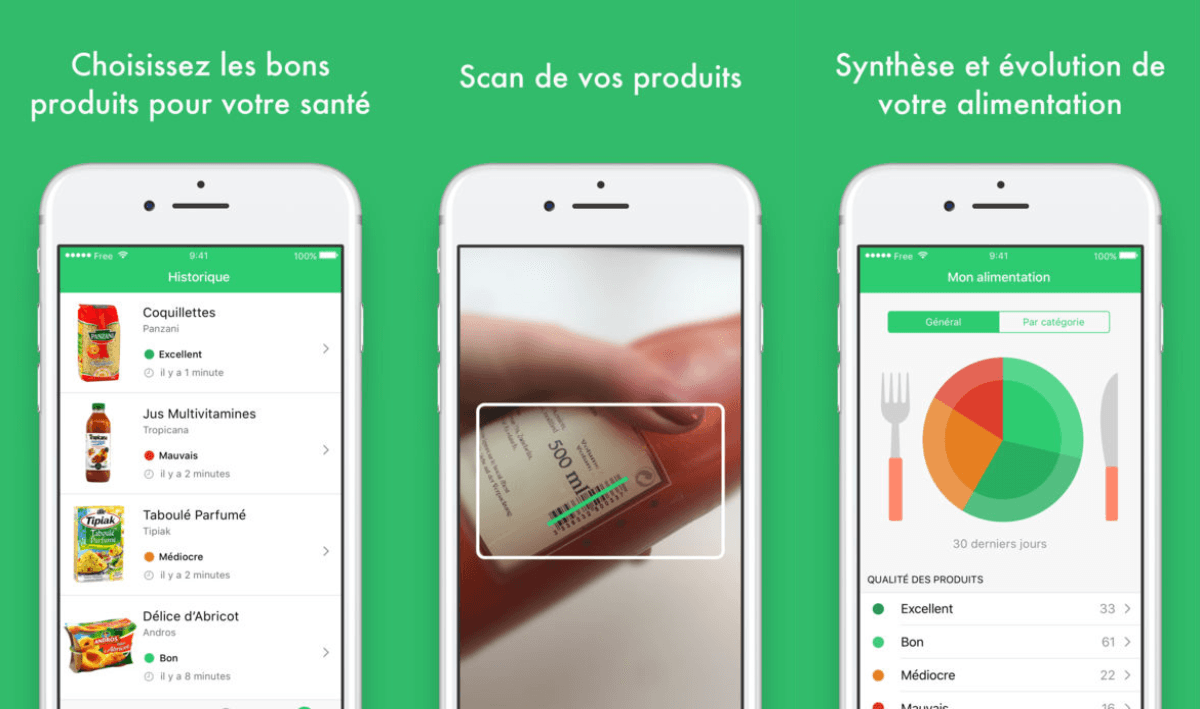
\includegraphics[scale=0.35]{images/yuka_evaluation.png}
\caption{The Yuka system for product evaluation}
\label{fig:yuka_evaluation}
\end{figure}
\end{center}
\par Its intuitive interface and simple scoring system based on composition,
additives, and organic status help users make quick purchasing decisions.
Despite these advantages, Yuka also presents notable limitations. Its
database is not always updated regularly. In addition, the application
lacks personalization by overlooking individual dietary goals, allergies,
and health conditions. As a result, Yuka serves more as a tool for initial
screening than as a source of personalized nutritional guidance.
\subsection{Open Food Facts}
Open Food Facts\footnote{\url{https://fr.openfoodfacts.org/}} is a collaborative and nonprofit database of food
products. It is the primary data source for many other applications,including Yuka. It is true that the Open Food Facts application provides transparent
information such as ingredients, allergens, and Nutriscore. But Open Food Facts suffers
from significant usability challenges. The lack of personal tracking or goal
setting features limits its usefulness for consumers seeking a nutritional
guide.
% OFF 00-01-02-03
\begin{figure}[H]
    \centering
    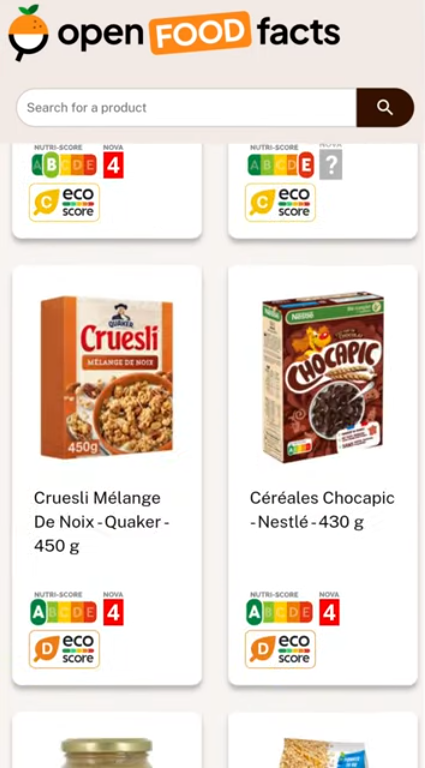
\includegraphics[width=0.24\textwidth]{images/OFF-00.png}
    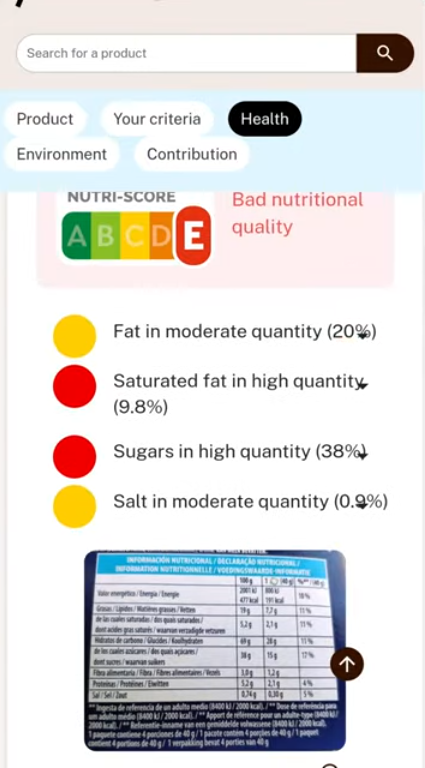
\includegraphics[width=0.24\textwidth]{images/OFF-01.png}
    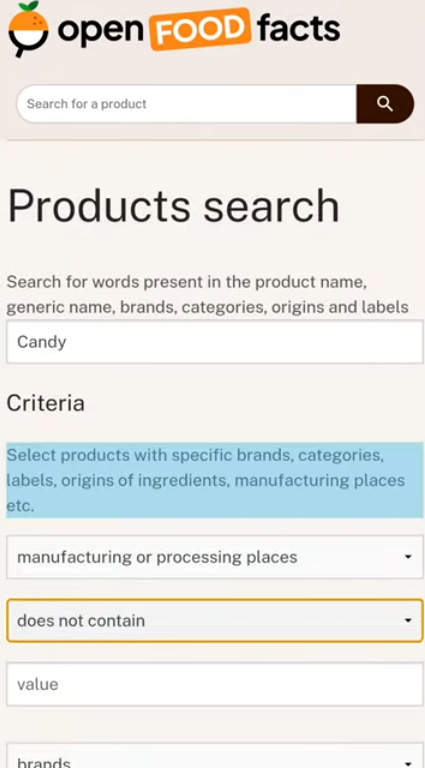
\includegraphics[width=0.24\textwidth]{images/OFF-02.png}
    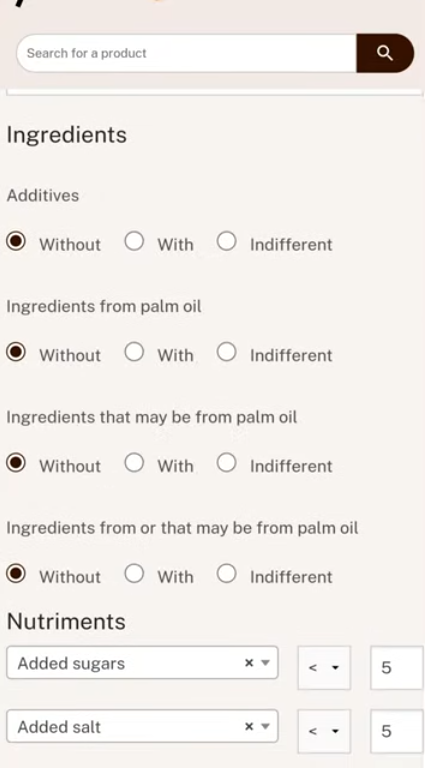
\includegraphics[width=0.24\textwidth]{images/OFF-03.png}
    \caption{Lack of personalization and user-friendly features in the OFF app}
    \label{fig:OFF_app}
\end{figure}

\subsection{QuelProduit}
\par QuelProduit\footnote{\url{https://www.quechoisir.org/application-mobile-quelproduit-n84731/}} is a product 
analysis application developed by the French non-profit consumer organization \textbf{UFC-Que Choisir} \footnote{\url{https://www.quechoisir.org/}}, to help users make
safer choices by scanning barcodes to evaluate food, cosmetic, and house-
hold items. 

 \begin{center}
\begin{figure}[H]
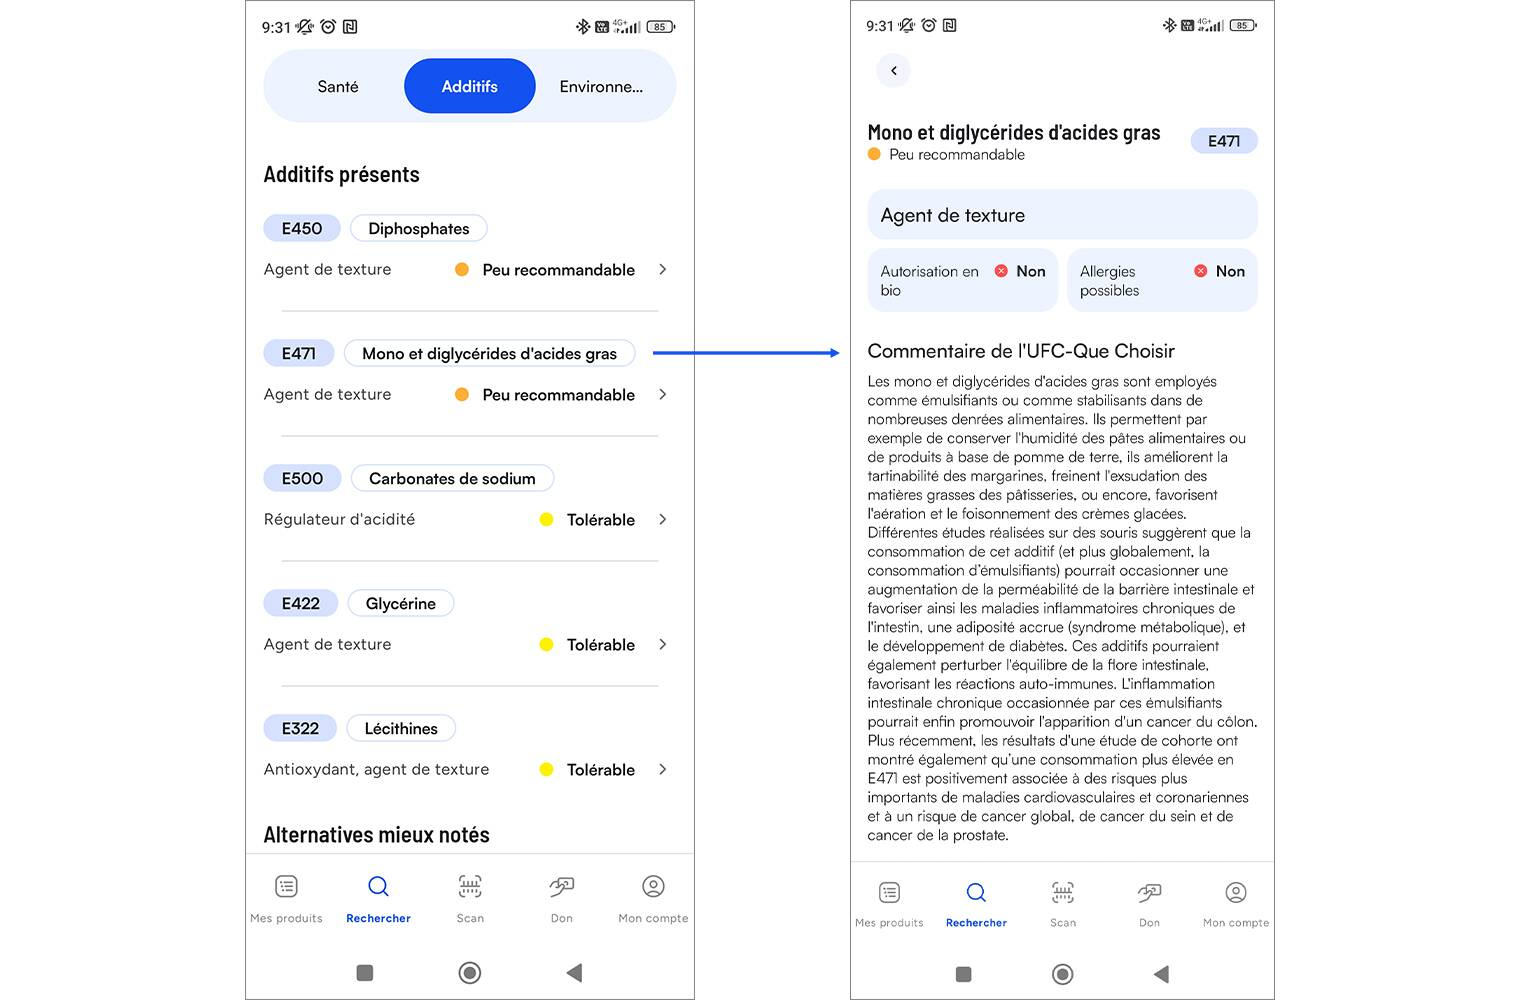
\includegraphics[scale=0.19]{images/quelproduit.jpg}
\caption{Identification of harmful substances and food additives by the QuelProduit application}
\label{fig:queChoisir}
\end{figure}
\end{center}

\par The application focuses on consumer safety by highlighting
harmful substances, but does not offer balanced nutritional guidance or
personalized dietary support. Users should view this tool as a simple
detection system rather than a nutritional guide or assistant.


\subsection{Food Check}
Food Check\footnote{\url{https://play.google.com/store/apps/details?id=com.bytes_and_pixels.food_buddy&hl=fr}} is an AI-powered nutritional scanner application developed by 
Bytes \& Pixels \footnote{\url{https://www.bytes-and-pixels.de/}}. The application offers AI chatbot assistance and personalized recommendations.

\begin{figure}[H]
\centering
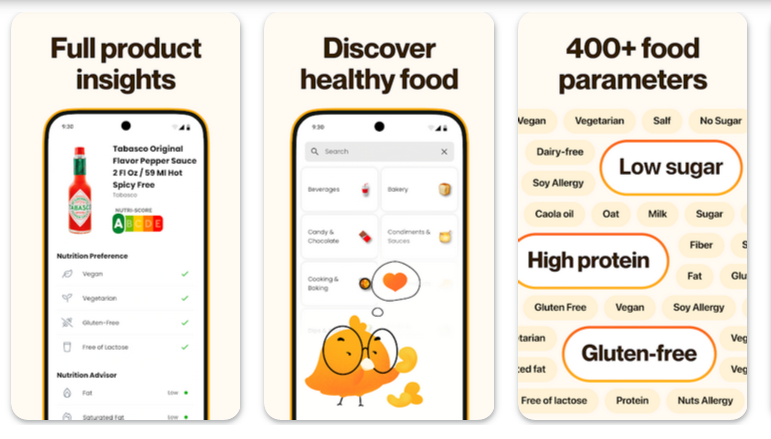
\includegraphics[scale=0.45]{images/food_check.png}
\caption{The complexity of parameters required from the user in the scanner application Food}
\label{fig:foofCheck}
\end{figure}

The main problem is the complexity of parameters to enter by user
to receive personalized recommendations. The onboarding process is
described as intrusive, requiring extensive personal information before
delivering value. This complexity can deter users from fully engaging
with the app, as illustrated in Figure\ref{fig:foodCheck}.

\subsection{Key Challenges and gaps in Current Applications}

There are a number of significant deficiencies of current nutritional apps.
The table\ref{tab:competitor_evaluation} summarizes the evaluation of key competitor applications
based on several criteria: frequency of database updates, recommendation
system sophistication, presence of a chatbot, level of user interaction,
and depth of product evaluation. This analysis highlights the strengths
and weaknesses of each application, providing a clear framework for
identifying opportunities to enhance VitamiNurse. Existing nutrition
applications frequently fall to deliver a comprehensive user experience.
Many provide basic recommendations by simple category-based filtering
that do not account for individual factors such as allergies and medical
conditions. This lack of personalization can make it difficult for users
to find relevant and actionable advice. Furthermore, the widespread
use of simplified scoring systems further reduces complex nutritional
data to a single value, which can mislead users and prevent informed
decision-making.
In the first three applications, there is a lack of interactivity. Real-time
chatbot guidance is missing to answer questions and provide tailored recommendations and advice. The lack of conversational guidance restricts
the ability of apps to provide dynamic and context-aware support.
For Food Check, this application does not consider user health conditions
evolution. The application requires users to input detailed personal information
during onboarding. This approach fails to adapt to changes in health status or dietary goals automatically over time, limiting long-term relevance
and effectiveness of recommendations.
% in Figure \ref{fig:yuka_feedback}. 

\begin{table}[htbp]
\centering
\small % Reduces font size to \small (you can also use \footnotesize for even smaller)
\caption{Evaluation of Key Competitor Applications}
\label{tab:competitor_evaluation}
\begin{tabularx}{1.15\textwidth}{|l|X|X|X|X|}
\hline
\textbf{Feature} & \textbf{Yuka} & \textbf{Open Food Facts} & \textbf{QuelProduit} & \textbf{Food Check} \\
\hline
Database Frequency Update & Not Frequent & Varies (by users) & Moderate & Moderate \\
\hline
Recommendation System & Elementary & Basic & Basic & Elementary \\
\hline
Chatbot & Absent & Absent & Absent & Present \\
\hline
Interaction & High & Moderate & Moderate & Moderate \\
\hline
Product Evaluation & Comprehensive & Comprehensive & Detailed & Detailed \\
\hline
\end{tabularx}
\end{table}


 
\section{Proposed Solution}
  
To address the identified market gaps, we propose a comprehensive
enhancement of the VitamiNurse application. Our vision is to transform it from a simple product scanner into an intelligent, adaptive, and
indispensable nutritional partner. This transformation is centered on delivering a uniquely personalized and interactive user experience through
the following key features.

\begin{figure}[H]
\centering
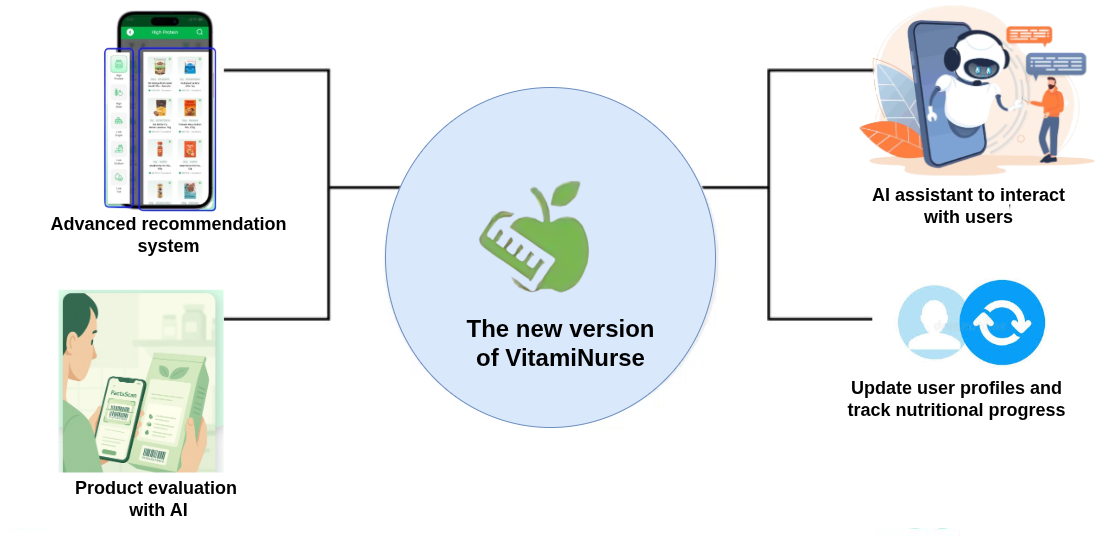
\includegraphics[scale=0.45]{images/new_version_VN.png}
\caption{Features of the new version of VitamiNurse}
\label{fig:VN_new_features}
\end{figure}

\subsection{An Interactive Nutritional Assistant}

To bridge the interactivity gap found in competing applications, VitamiNurse will feature a friendly AI assistant integrated directly into the
user experience.
\par This 24/7 assistant serves as a conversational partner
for all nutritional inquiries, providing dynamic support that goes beyond
simple question–answer chatbots.
The assistant will be capable of answering a wide range of questions,
from clarifying nutritional information to offering meal suggestions based
on preferences and dietary restrictions of each user.

\subsection{Personalized Product Recommendations}
We recognize that nutritional needs are highly individual. Moving beyond
generic scoring systems, VitamiNurse will provide deeply personalized
guidance. The application learns from user preferences, dietary restrictions, and health goals to offer tailored product recommendations.
For example, if a user is managing hypertension, the application will prioritize low-sodium options when suggesting alternatives to scanned products. 
This level of personalization ensures that users receive relevant and actionable advice that aligns with their unique health profiles.

\subsection{Product Evaluation Using AI}

The application functions as a personal nutritionist at the point of sale.
It transcends simply listing ingredients by performing a sophisticated
evaluation tailored to the user’s unique health profile, whether it be for
weight management, diabetes, or hypertension.


\subsection{Continuous Updates of Product Database and User Profiles}

A fundamental limitation of existing applications is the lack of current
and accurate product information. Our solution ensures that users can
have complete confidence in the data they access. The system is designed
to automatically and continuously refresh its database by using a data
pipeline from trusted sources.
Without the need for manual updates, the application will maintain
dynamic user profiles in real-time that evolve with the user’s health
status and dietary goals. This adaptability ensures that recommendations
remain relevant over time, accommodating changes in lifestyle, health
conditions, and personal preferences. By continuously updating both
product data and user profiles, VitamiNurse aims to provide a truly
personalized and trustworthy nutritional guidance experience.


\section{Comparative Study of existing methodologies}

The first step to ensure the smooth running and success of any project
is choosing the right methodology. Today,Scrum, XP, and Kanban and
Scrumban are the most popular agile approaches in web and mobile
development. To choose the best approach, we decided to compare and
select the one that best fits our context and objectives.

\subsection{Scrum Method} 


\par Scrum is an agile methodology that promotes collaboration, adaptability, and the iterative delivery of high-quality results. This method encourages agile teams to meet regularly to review project progress and adjust their direction as needed. This dynamic approach balances investment and the final product, ensuring greater customer satisfaction and optimal value delivery \cite{scrum2025}.
The main elements of Scrum are:

\begin{enumerate}[label=\textbf{-}]
    \item \texttt{Sprint:} Is a working cycle with fixed duration, of one to four weeks. In this case, it is the Scrum Master to ensure that this period is not exceeded \cite{schwaber2004agile}

    \item \texttt{Scrum Master:} Their main role is to facilitate the application of Scrum principles and resolve blockages.

    \item \texttt{Scrum Team:} A multidisciplinary, self-organizing team that manages the planning and delivery of features.


    \item \texttt{Product Owner:} He validates the functionalities, prioritizes the requirements and user expectations.

    
\end{enumerate}
\subsection{Kanban Method}
Kanban, originating from Japanese industry, is a visual workflow management tool. It allows you to visualize and limit work in progress in software development and IT work . The main elements of Kanban are as follows:

Kanban, originating from Japanese industry, is a visual workflow management tool. It allows you to visualize and limit work in progress in software development and IT work\cite{anderson2010kanban}. The main elements of Kanban are as follows:A \texttt{Kanban board} visualizes workflow steps ("To do", "In progress", "Done"), \texttt{Kanban cards} represent tasks with their details (description, deadlines), and \texttt{WIP} (Work In Progress) reduces overloads and quickly identifies bottlenecks.

\subsection{XP Method (eXtreme Programming)}

XP takes agile principles to the extreme with rapid iterations and enhanced customer collaboration with minimal documentation. It is characterized by frequent code reviews and a creative and collaborative working environment through pair programming\cite{beck2000extreme}. 


By performing frequent code reviews and unit tests to make changes quickly, it seeks the best quality and customer satisfaction that remains in constant contact throughout the project. This approach is based on 5 values: \texttt{Simplicity}, which is favored by the search for easier solutions to achieve objectives; \texttt{communication} in direct communication between team members on the one hand and the client on the other; \texttt{feedback} through the constant exchange of feedback between the project team and key customers; \texttt{courage} required to undertake changes such as exploring new paths; and \texttt{respect} for each team member and their work.


\subsection{Scrumban Method}
Scrumban is a hybrid methodology that combines the flexibility of Kanban board with the rigor of Scrum sprints. Scrum roles are incorporated while enabling real-time modifications and the best possible workflow visualization. The team does, in fact, follow certain rituals, use sprints, and assign roles to the Scrum Master and Product Owner. Nonetheless, the procedure is less exacting than Scrum, enabling teams to maintain an ideal workflow and make real-time priority adjustments.

\begin{center}
\begin{figure}[H]
            \centering
            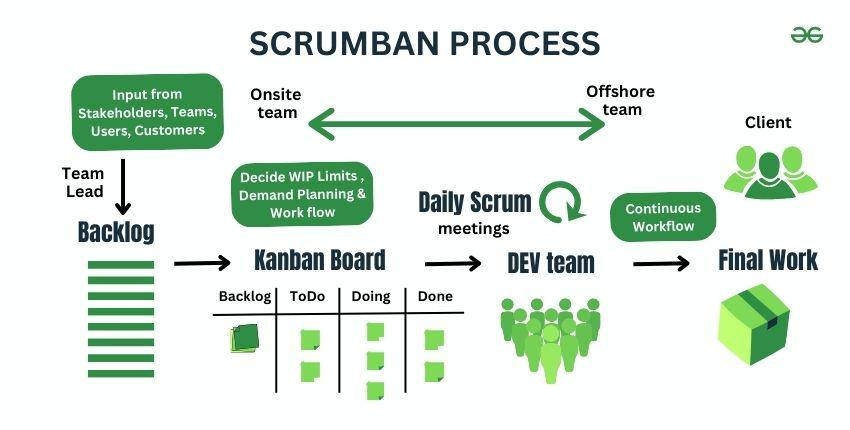
\includegraphics[scale=0.55]{images/scrumban.jpg}
            \caption{Scrumban Process }
            \label{fig:Scrumban_Process}
\end{figure}
\end{center}   


\section{Team Management Methodology}
Our selection of the \textbf{Scrumban} methodology is based on an analysis of the limitations of pure approaches (Scrum, XP, Kanban) in the practical plan in the host company as well as the specific needs of our project. Generally, we can summarize the identified problems as follows:
\begin{itemize}
    \item \textbf{Limited numbers:}
    The XP (eXtreme Programming) approach requires development pairs (pair programming), which is difficult to apply with the available human resources.
        Project planning
    \item \textbf{Accelerated Scrum Pace:}
    Short sprints (2–4 weeks) can generate excessive pressure on the development team, risking compromising quality, especially for an end-of-study internship.    
        
    \item \textbf{Flexibility needs:}
    The rigidity of Scrum rituals (mandatory sprint planning) is unsuitable for the rapid evolution of artificial intelligence technologies and the frequent changes imposed by stakeholders.
    \end{itemize}
    
\par Scrumban effectively addresses these challenges by combining Scrum's structured framework with Kanban's flexibility. This hybrid approach allows us to maintain essential Scrum elements, such as defined roles and sprint planning, while incorporating Kanban's visual workflow management and adaptability. This balance is particularly beneficial for our project, which requires both structure and the ability to respond quickly to new insights and technological advancements.
The first step in the Scrumban process is to set up the Scrumban board, which is an enhanced version of the Kanban board. It contains all the features, including the product backlog, sprint backlog, and workflow stages (not started, in progress, and under review). The Scrumban board allows us to visualize the entire workflow, track task progress, and identify bottlenecks in real time. 
\section{Chosen technical methodology}

For the technical execution, we adopted the CRISP-DM for its structured
and iterative approach to solving complex data science problems. It
represents a comprehensive six-phase process includes problem understanding, data exploration, data preparation, modeling, evaluation, and
deployment.
\begin{center}
\begin{figure}[H]
            \centering
            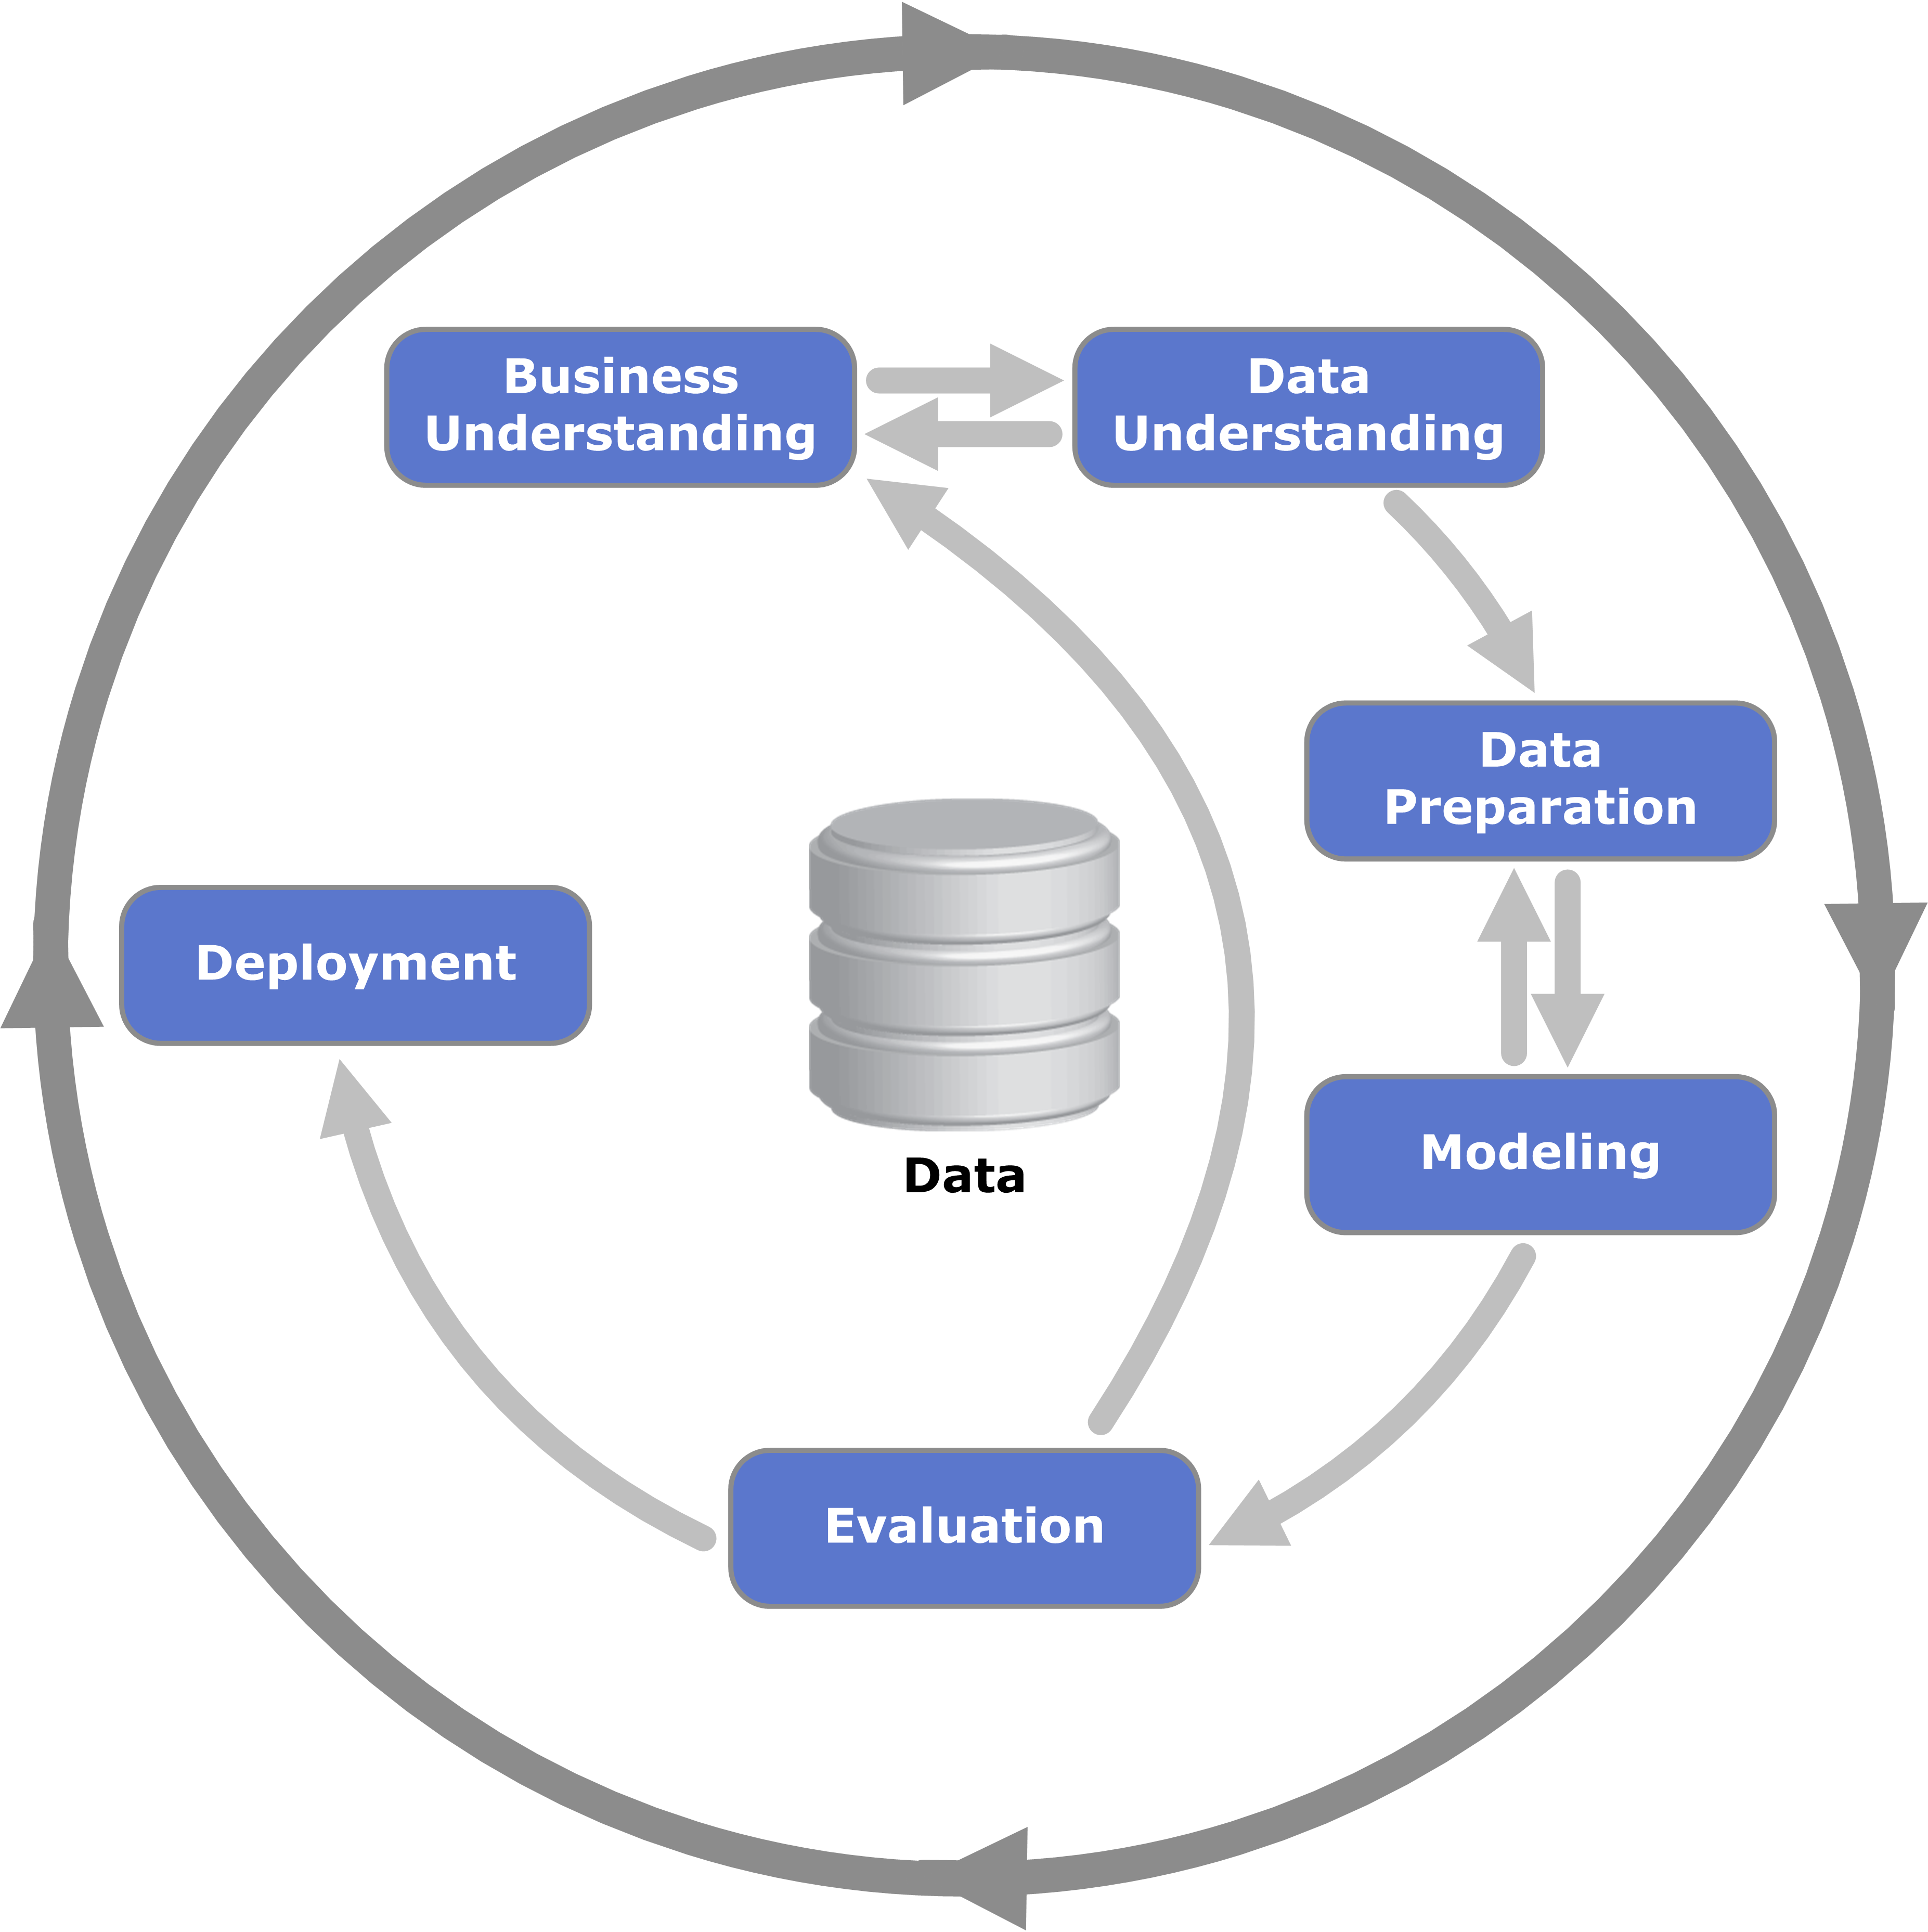
\includegraphics[scale=0.44]{images/CRISP.png}
            \caption{CRISP-DM} 
            \label{fig:CRISP_DM}
        \end{figure}
\end{center}

\par This methodology is particularly well-suited for our project, which involves
developing a personalized recommendation system and an AI assistant
for nutritional guidance. The structured phases of CRISP-DM allow
us to systematically address the challenges of data collection, model development, and deployment while ensuring that we remain aligned
with user needs and project goals.



\section{Project Planning}

This section details the strategy for enhancing the VitamiNurse application over a period of nine months. 
In alignment with our chosen Scrumban approach, we can maintain a structured workflow while staying flexible enough to adapt to new insights.
Using our Scrumban board, as shown in Figure~\ref{fig:Tableau_Scrumban}, we maintain clear visibility of progress and quickly identify any bottlenecks in the development process.


\begin{center}
\begin{figure}[H]
            \centering
            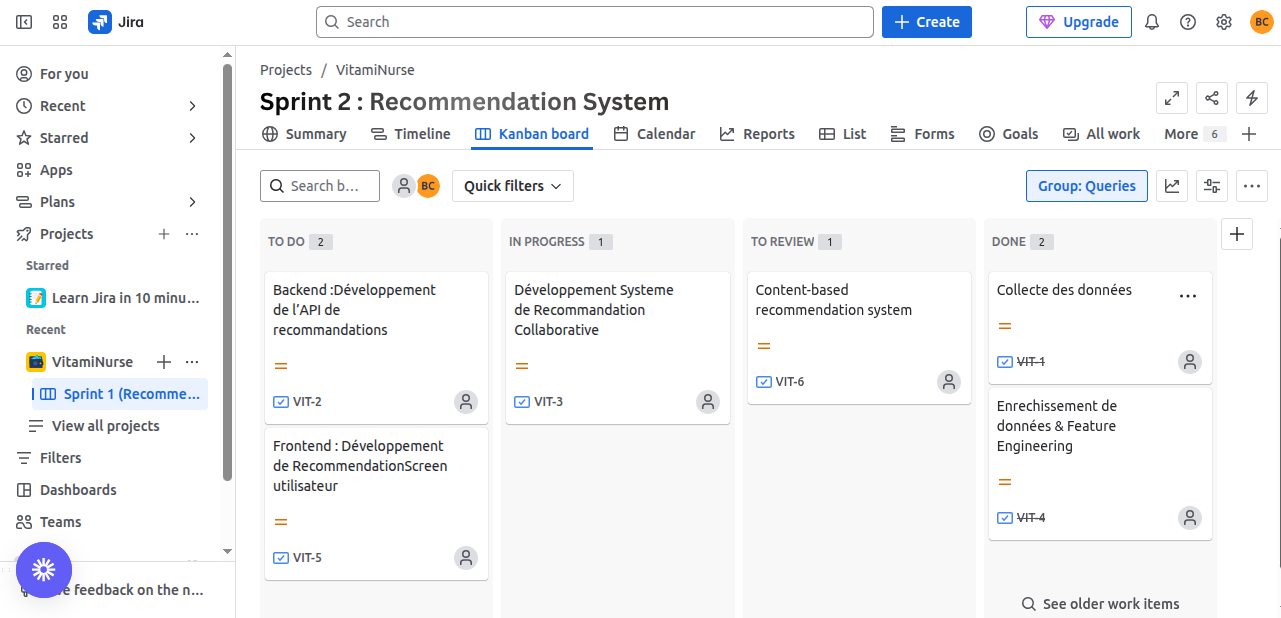
\includegraphics[scale=0.55]{images/kanbanBoard.png}
            \caption{Our Scrumban Board Implementation}
            \label{fig:Tableau_Scrumban}
\end{figure}
\end{center}

\subsection{Development Approach}

 Our process is divided into three distinct phases, each lasting three months and composed of six two-week iterations.
This structure provides the necessary framework while allowing us to adapt to emerging challenges in our artificial intelligence and machine learning components. 
\begin{figure}[H]
\centering
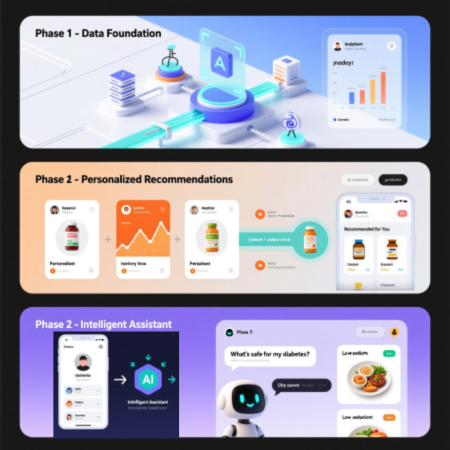
\includegraphics[scale=0.72]{images/planning.png}
\caption{Project Phases}
\label{fig:project_timeline}
\end{figure}

\subsection{Project Management with Jira}

To effectively implement our Scrumban methodology, we adopted \textit{Jira} as the central project management platform. Jira provides native support for hybrid agile frameworks, enabling us to configure a customizable Scrumban board that reflects our workflow stages: \textit{Backlog}, \textit{Ready}, \textit{In Progress}, \textit{In Review}, and \textit{Done}. 

Each user story and technical task is documented as a Jira issue, tagged with epics corresponding to the three project phases, and assigned to team members with clear deadlines aligned with two-week iterations.
Given the complexity of our AI-driven features and the need for rigorous version control and task accountability, Jira’s scalability, extensibility, and alignment with software engineering best practices make it the optimal choice for managing the VitamiNurse enhancement project \cite{atlassian2023jira}.


\subsection{Phase One: Building a Reliable Data Foundation (Months 1-3)}

The initial phase addresses a critical weakness identified in our competitive analysis: incomplete and outdated product information. We focus on building a reliable data infrastructure to ensure comprehensive and current nutritional information. Our technical implementation consists of an automated data pipeline that performs daily updates from trusted nutritional databases, complemented by a machine learning model for predicting missing nutritional values. 
Users receive complete nutritional information for all products, which helps users to make informed dietary choices. Our key deliverables include an operational data collection pipeline and trained nutritional prediction models. We measure success through maintaining daily database updates and ensuring mean absolute error less than 10\% on predicted nutritional values

\subsection{Phase Two: Creating a Personalized Recommendation Engine (Months 4-6)}

Building on our robust data foundation, we develop an advanced recommendation system that delivers personalized product suggestions. 
This directly addresses the personalization limitations found in competitor applications, as highlighted in Table~\ref{tab:competitor_evaluation}. 
Our system combines content based and collaborative filtering techniques to provide more sophisticated recommendations than existing solutions.

The implementation creates detailed user profiles incorporating health conditions, dietary restrictions, personal preferences, and nutritional goals. Our hybrid recommendation algorithm analyzes both product attributes and user behavior patterns, including scans, preferences, and viewing history to continuously refine suggestions. Technical deliverables encompass the recommendation engine backend, user interaction tracking, and intuitive interfaces for displaying personalized suggestions.

\subsection{Phase Three: Developing an Intelligent Assistant (Months 7-9)}

In the final phase, we will introduce a conversational assistant powered by a RAG pipeline and large language models (LLMs). 
This addresses the interactivity gap in the current market and transforming VitamiNurse into a comprehensive nutritional partner. The smart evaluation system will use AI to analyze any product against the individual health profile of the user. 
Implementation focus on developing the AI evaluation system, integrating the conversational assistant, and creating user-friendly interfaces for interaction.


\subsection{Risk Management and Progress Strategy}

Our phased approach minimizes technical and project risks by validating each component before advancing to more complex features. The solid data foundation from Phase 1 reduces risks in recommendation system development, while both initial phases prepare essential infrastructure for our AI assistant. 

Regular reviews and demonstrations align with our Scrumban methodology, allowing us to adjust priorities based on stakeholder feedback and emerging insights. This structured approach ensures our nine month internship delivers meaningful progress in transforming VitamiNurse into a competitive, intelligent nutritional application. 
Each phase produces tangible value while building toward our complete vision, directly addressing the market opportunities identified in our comprehensive competitor analysis.


\section*{Conclusion}
\addcontentsline{toc}{section}{Conclusion}
In this first chapter, we presented the context of our internship project
at ONRTECH, focusing on the development of a new version of the VitamiNurse application.
We analyzed existing nutritional applications to identify their
strengths and weaknesses, which informed our proposed enhancements
for this project. Our solution leverages more artificial intelligence to
improve user nutritional support through an advanced recommendation system and a
user-friendly AI assistant. The methodological framework for the project was also defined,
 combining Scrumban for project management and CRISP-DM for the technical data science workflow. 
 Collectively, this chapter provides the necessary foundation for the subsequent phases of this work, 
 which will detail the design and implementation of the new features of VitamiNurse.
\chapter{Nutri-pred-v1: A Model for Nutrition Value Prediction}

\section{Introduction}
\par In the VitamiNurse project, automated completion of missing nutritional
values represents a critical challenge. The primary data source relies
on web scraping, which frequently yields products with incomplete or
missing nutritional information. This section details the development
and evolution of the machine learning model Nutri-pred-v1, specifically
designed to address this need by automatically predicting nutritional
values of food products from their names and textual descriptions.
\par The model leverages a large dataset of food products from Open Food
Facts with varying degrees of nutritional information completeness. The
goal is to create a robust predictive model capable of accurately estimat-
ing key nutritional attributes such as energy (kcal), fat, saturated fat,
carbohydrates, sugars, proteins, and salt based solely on product names
and descriptions.
\section{Data Acquisition and Initial Setup}
The Open Food Facts (OFF) is a collaborative and open-access database
that contains information of more than 3.8 million food products. This
global dataset, which includes products from many countries as shown in
the bar chart in Figure 2.1, can be downloaded in its entirety in either
CSV or JSON formats. Because of its extensive size (11.4 GB) and the
high dimensionality of the data, it is essential to optimize memory usage
during data preprocessing.

\par An effective and widely used technique in data science consists of loading
only the columns needed for training the model. This selective loading
approach significantly reduces memory consumption and processing time.
The dataset contains a wide range of attributes, including product names,
ingredients, brands, categories, and detailed nutritional information.
\par However, many entries have missing or incomplete nutritional profiles,
which poses a challenge for model training. To address this, we focused on
products that have complete nutritional information for the key attributes
we aim to predict.

\begin{figure}[H]
\centering
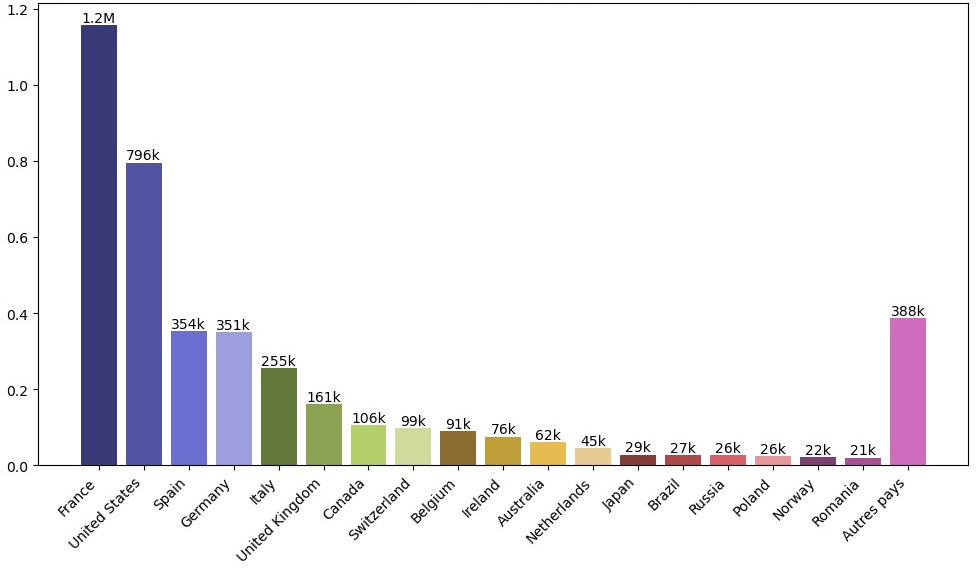
\includegraphics[scale=0.45]{images/OFF_database.png}
\caption{Distribution of food products in the Open Food Facts database by country of origin} 
\label{fig:country_distribution}
\end{figure}

\section{Data Exploration and Cleaning}
Because of the collaborative nature of the dataset, many problems can be encountered. It require substantial cleaning and preprocessing efforts in order to ensure reliability of our data.
These problems include :

\begin{itemize}[label=\textbf{-}]
\item \textbf{Missing Values:} Many entries have incomplete nutritional profiles, which affects the ability to use them for training ML models.
\item \textbf{Inconsistent and Erroneous Values:} Some fields contain inconsistent or obviously erroneous values due to unit or user input errors .
\item \textbf{Negative Values:} Several nutritional values are negative, which is physiologically unrealistic.
\end{itemize}


\subsection{Initial Dataset Overview}
The initial dataset comprised 3,800,000 products. After preprocessing and cleaning, the dataset was reduced to 2,225,014 products.
This refinement process ensured that all entries had complete textual descriptions, contained non-null and plausible nutritional values, and featured homogenized units to guarantee consistency across the entire dataset.
The collaborative nature of Open Food Facts introduces several data quality challenges that must be addressed before model training.

\begin{figure}[H]
\centering
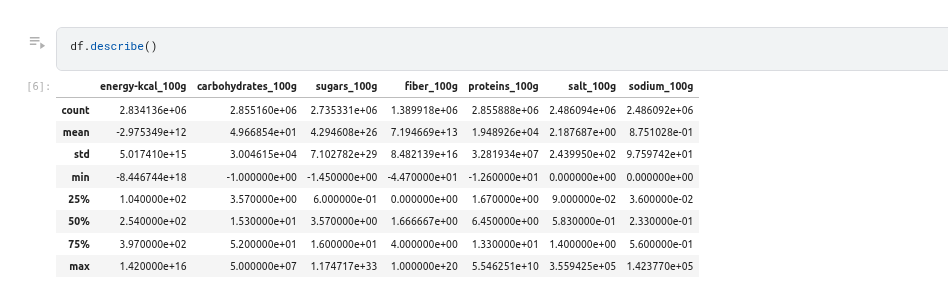
\includegraphics[scale=0.55]{images/statistics.png}
\caption{Explore data statistics} 
\label{fig:data_statistics}
\end{figure}

\subsection{Handling Missing Data}
To address the challenge of missing data, we adopt a selective retention. Features with high missingness, such as energy-kJ  (missing >86 \%) and fiber (missing >52 \%), are excluded in order to preserve data integrity and avoid imputation bias. 
\par In contrast, the other nutritional features (energy-kcal, fat, carbohydrates, and proteins) are retained due to their low missingness rates  ($<$ 3.3\%) and critical role in nutritional modeling \cite{stoian2020machine}.
This selective retention ensures a robust and representative set of features in order to guarantee an effective model training.

\begin{figure}[H]
\centering
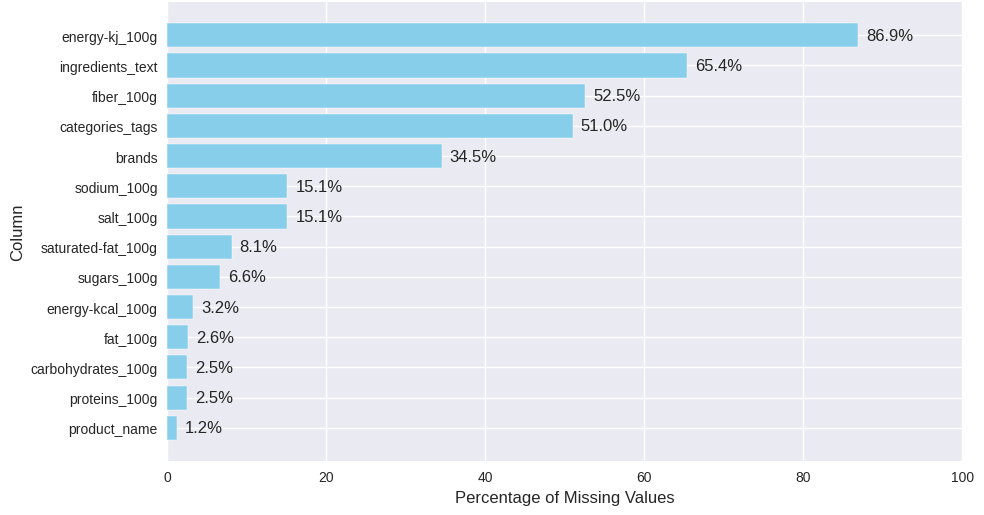
\includegraphics[scale=0.51]{images/missing_values.png}
\caption{Proportion of missing values} 
\label{fig:missing_values}
\end{figure}

\subsection{Filtering Implausible Nutritional Values}
This filtering step was implemented in order to remove entries with implausible nutritional values, such as negative calories or excessive amounts of nutrients. These errors can distort  the performance any machine learning model. We defined plausible nutritional ranges for each nutrient per 100g of product. These thresholds reflect chemically realistic limits. 
For example,  900 kcal represents the upper physiological limit for energy content in food composed solely of fat, such as oils. This theoretical maximum energy is calculated based on the Atwater general factor system that includes energy values of 4 kcal per gram (17 kJ/g) for protein, 4 kcal/g for carbohydrates and 9 kcal/g (37 kJ/g) for fat \cite{huelEnergyCalculation}.

Thus the total energy content per 100 grams can be estimated using the following formula:
$$
\text{Energy (kcal/100g)} = 4 \times (\text{g carbs}) + 4 \times (\text{g proteins}) + 9 \times (\text{g fats})
$$

The theoretical maximum energy density is reached when a product consists entirely of fat, as it yields the highest caloric value per gram. In this case, the energy content is:
\[
\text{Energy} = 9 \times 100 = 900 \text{ kcal/100g}
\]
The process then continues with all the other macronutrients like it is illustrated in the provided table to retain only nutritionally realistic entries.
% Creating the table for nutritional ranges
\begin{table}[H]
\centering
\caption{Plausible Nutritional Ranges for Data Validation in product Composition per 100g}
\resizebox{0.75\textwidth}{!}{%
\begin{tabular}{@{}lcp{10cm}@{}}
\toprule
\textbf{Nutrient} & \textbf{Plausible Range} & \textbf{Scientific Rationale and Validation Criteria} \\
\midrule
Energy & 0--900 kcal & Energy content is derived from the Atwater system by employing the 4-9-4 method: carbohydrates, proteins and fats. The theoretical maximum of $\sim$900 kcal/100g occurs in pure fats like oils. \\  \\
Carbohydrates & 0--100 g & Includes sugars, starches, and dietary fiber, expressed as a mass fraction. Pure carbohydrate sources like sugar and starch may approach 100 g/100g, constrained by total mass . \\ \\
Total Fat & 0--100 g & Represents all lipid fractions. Pure fats like olive oil and butter may reach 100 g/100g, validated by gravimetric methods like Soxhlet extraction. \\ \\
Saturated Fat & 0--100 g & A subset of total fat, limited by total fat content. Pure saturated fat sources such as coconut oil may reach 100 g/100g, quantified via gas chromatography . \\ \\
Sugars & 0--100 g & Includes mono- and disaccharides. Pure sugar products (e.g., sucrose, honey) may reach 100 g/100g. \\ \\
Proteins & 0--90 g & Limited by food matrix composition. High-protein foods like whey protein and dried meat may approach 90 g/100g, quantified by Dumas methods \cite{moore2022}. \\ \\
Salt & 0--30 g & Constrained by sensory acceptability and public health recommendations outlined by the World Health Organization (WHO) regarding sodium intake \cite{who2012}. \\
\bottomrule
\end{tabular}
}
\label{tab:nutritional_ranges}
\end{table}
\vspace{0.4cm}

\subsection{Data Cleaning and Deduplication}
To ensure data integrity and eliminate redundancy, we identified and removed \textbf{1604} fully duplicated rows in the dataset to ensure that each product instance is unique.
\par Additionally, since the product name is a critical textual feature for nutritional prediction, we discarded \textbf{23,740} rows with missing values in the product\textunderscore name field to guarantee meaningful and consistent textual representations. For the training process, only the product\textunderscore name field was vectorized using the TF-IDF (Term Frequency–Inverse Document Frequency) approach to extract relevant textual features for modeling.

\section{Feature Engineering}

\subsection{Feature Selection Strategy}
The feature selection strategy for our high-dimensional nutritional dataset integrates established machine learning principles to enhance model robustness. This approach, combining correlation-driven dimensionality reduction, missing  informed-data exclusion, and unit consolidation, optimizes predictive performance while preserving essential information. This step is important to ensure effective model training while preserving critical nutritional information.

\subsubsection{Correlation-Driven Feature Exclusion}
To mitigate redundancy and numerical instability, we exclude features exhibiting near-perfect correlation. Following Guyon and Eliseeff (2003) \cite{guyon2003}, the feature energy-kJ\_100g is removed due to its perfect negative correlation ($r \approx -1$) with energy-kcal\_100g. Including both variables provides no additional predictive information and risks numerical instability in model training due to multicollinearity. Instead, we retain energy-kcal\_100g and leverage the thermodynamic conversion factor:
$$1~\mathrm{kcal} = 4.184~\mathrm{kJ}$$

This expression is used to derive energy-kJ\_100g post-training, ensuring computational stability and preserving predictive accuracy.

% Creating the table for nutritional ranges
\begin{figure}[H]
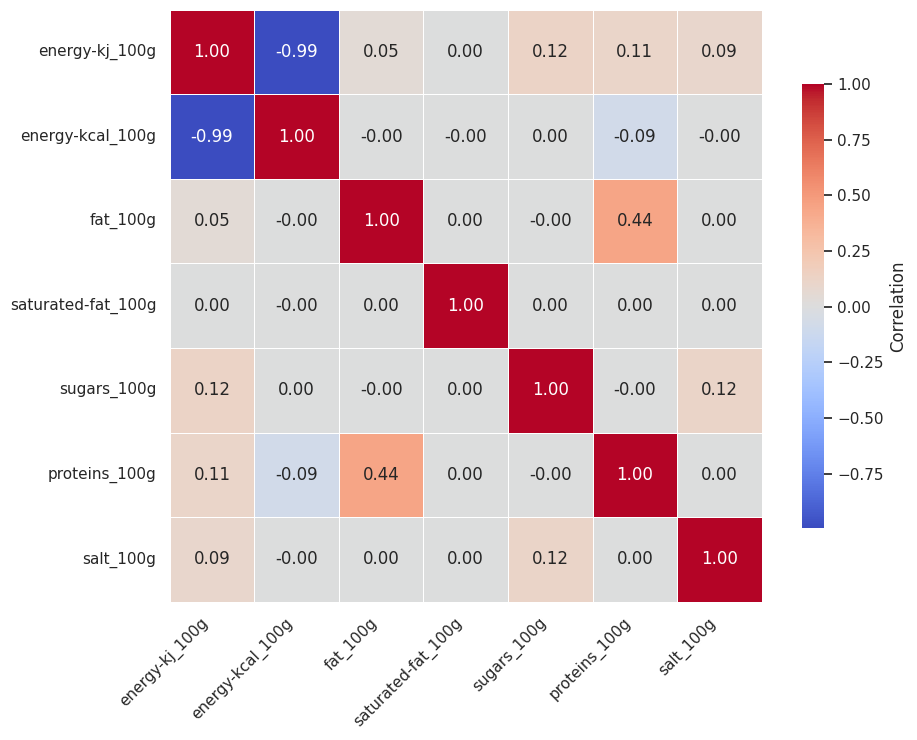
\includegraphics[width=0.9\textwidth]{images/correlation_matrix.png}
\caption{Correlation matrix} 
\label{fig:Correlation_matrix}
\end{figure}

\subsection{Text Vectorization with TF-IDF}
The preprocessing phase was designed to ensure data consistency and compatibility. In order to maintain data integrity, text cleaning was done first. This included the removal of special characters, normalize text case to ensure uniformity , and systematic process missing or inconsistent text fields . Text descriptions were then vectorized using the Term Frequency-Inverse Document Frequency (TF-IDF) approach in order to extract features. This process transformed the text data into numerical representations, limiting the feature set to a maximum of 12,000 features  to optimize computational efficiency and model performance. This choice will be proved later in the Hyperparameter Tuning step ~\ref{tab:max_features_values}.

\subsection{TF-IDF Hyperparameter Optimization}
A machine learning pipeline was developed, integrating a Term Frequency-Inverse Document Frequency (TF-IDF) Vectorizer with a multi-output regression model to predict nutritional attributes from the product\_name, aligning with established natural language processing practices.
\par To optimize performance, a grid search with 3-fold cross-validation was conducted to determine the optimal \texttt{max\_features} parameter for the TF-IDF Vectorizer, ensuring robust model evaluation \cite{hastie2009elements}. The following configurations were evaluated:

\begin{itemize}
    \item \textbf{Base Regressor}: Linear Regression was selected as the foundational model for the multi-output regression task, leveraging its simplicity and effectiveness in high-dimensional settings, consistent with the dataset's characteristics.
    \item \textbf{Hyperparameter Tuning}: The \texttt{max\_features} parameter of the TF-IDF Vectorizer was tuned over different values ranging from 500 to 15000 , following standard approaches for optimizing feature selection in text-based nutritional prediction \cite{aionlinecourse2025}.
\end{itemize}

\par As shown in the previous table\ref{max_features_values} the grid search identified the optimal configuration with \texttt{max\_features = 12000}. By achieving a Mean Absolute Error (MAE) of 18.76,it demonstrates effective predictive performance for the nutritional attributes. While increasing the number of features consistently improved accuracy, gains became marginal beyond 12000, suggesting this value offers a good balance between complexity and performance.

\begin{table}[H]
\centering
\caption{Comparison of Mean Absolute Error (MAE) for Different \texttt{max\_features} Values}
\begin{tabular}{cS[table-format=5.0]S[table-format=2.4]S[table-format=1.4]}
\toprule
{Fold} & {\texttt{max\_features}} & {MAE} & {Standard Deviation} \\
\midrule
1 & 500 & 23.6168 & 0.0169 \\
2 & 1000 & 22.1044 & 0.0069 \\
3 & 2000 & 20.6975 & 0.0255 \\
4 & 3000 & 20.0193 & 0.0029 \\
5 & 5000 & 19.3171 & 0.0131 \\
6 & 6000 & 19.1467 & 0.0058 \\
7 & 7000 & 19.0157 & 0.0149 \\
8 & 8000 & 18.9249 & 0.0086 \\
9 & 9000 & 18.8800 & 0.0109 \\
10 & 10000 & 18.8278 & 0.0037 \\
11 & 12000 & 18.7647 & 0.0193 \\
12 & 14000 & 18.7665 & 0.0222 \\
13 & 15000 & 18.7676 & 0.0248 \\
\midrule
\multicolumn{2}{l}{\textbf{Best Parameter}} & \multicolumn{2}{l}{\texttt{max\_features} = 12000} \\
\multicolumn{2}{l}{\textbf{Best MAE}} & \multicolumn{2}{l}{18.7647} \\
\bottomrule
\end{tabular}
\label{tab:max_features_values}
\end{table}

\section{Model Construction and Training}
After finishing preprocessing and feature engineering, we built a supervised learning pipeline to predict seven key nutritional attributes from product text. The next subsections summarize the model architecture, hyperparameter tuning, and evaluation procedures used to build Nutri-pred-v1.

\subsection{Training Set Construction}
A stratified random sample of 10\% of the dataset (222,501 products) was selected to perform model experimentation and hyperparameter tuning. The target variables were the following nutritional attributes: energy (kcal), fat, saturated fat, carbohydrates, sugars, proteins, and salt.
Entries with missing values in any of these target variables were removed to ensure reliable supervision during training.

\subsection{Model Architecture and Algorithm Selection}
Trained on a large dataset of 2.2 million products and demonstrating strong generalization with satisfactory accuracy, the model Nuti-prd-v1 utilized a MultiOutputRegressor based on KNeighborsRegressor (n\_neighbors=5, n\_jobs=-1). It is selected after comparative evaluation of multiple multi-output regression algorithms trained on the complete Open Food Facts dataset. This configuration, designated Nutri-pred-v1, minimized the mean absolute error (MAE) on nutritional variables.

\begin{itemize}[label=-]
    \item \textbf{Input}: TF-IDF vectors (12,000 features) derived from product names and descriptions
    \item \textbf{Output}: Predictions for 7 nutritional variables
    \item \textbf{Energy calculation}: energy\_kj\_100g = energy\_kcal\_100g × 4.184
    \item \textbf{KNN rationale}: Selected for its capacity to capture nonlinear relationships in high-dimensional TF-IDF space, demonstrating superior MAE performance among tested models
\end{itemize}

\section{Model Evaluation and Selection}

\subsection{Comparative Model Analysis}
\par This step we evaluate the effectiveness of various machine learning algorithms for predicting nutritional values, a comprehensive comparative analysis was conducted. This study assessed the performance of multiple regression models, including K-Nearest Neighbors (KNN), Linear Regression, CatBoost, LightGBM, XGBoost, and Random Forest.
% Including figure for model comparison
\begin{figure}[H]
    \centering
    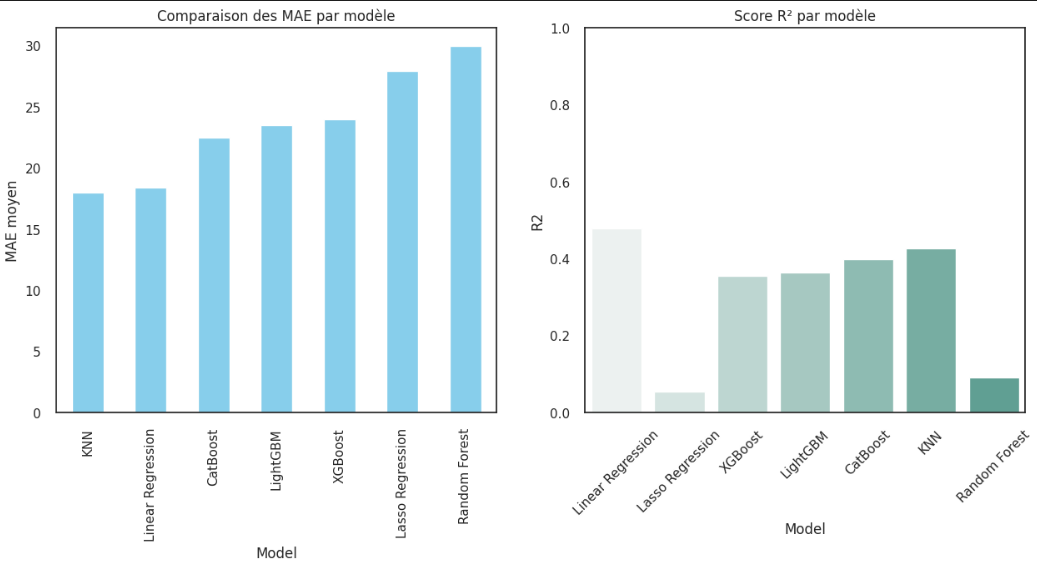
\includegraphics[width=0.98\linewidth]{images/mae_r2_comparison.png}
    \caption{Comparison of Mean Absolute Error (MAE) and \(R^2\) across regression models.}
    \label{fig:model_comparison}
\end{figure}

The performance of each model was quantified using two key metrics: Mean Absolute Error (MAE) and coefficient of determination ($R^2$) that offer critical insights into model accuracy and explanatory power. The results are summarized in the table~\ref{tab:model_results}, with MAE and \(R^2\) values for each algorithm.

\begin{table}[H]
    \centering
    \caption{Performance metrics of regression models}
    \begin{tabular}{lcc}
        \toprule
        \textbf{Model} & \textbf{MAE} & \textbf{\(R^2\)} \\
        \midrule
        K-Nearest Neighbors & 17.939 & 0.427 \\
        Linear Regression & 18.396 & 0.478 \\
        CatBoost & 22.472 & 0.397 \\
        LightGBM & 23.499 & 0.364 \\
        XGBoost & 23.948 & 0.354 \\
        Lasso Regression &  27.933 & 0.055 \\
        Random Forest & 29.955 & 0.090 \\
        \bottomrule
    \end{tabular}
\end{table}

\subsection{Performance Metrics and Model Selection}
 The K-Nearest Neighbors (KNN) model achieved the lowest MAE of 17.94, indicating high predictive accuracy with minimal average deviation between predicted and actual values. Its \(R^2\) of 0.427, while reasonable, is slightly lower than Linear Regression's 0.478, which captures a marginally higher proportion of variance. 
 \par Other models, including CatBoost , LightGBM , XGBoost , and Random Forest , exhibited higher errors and lower explanatory power, with Random Forest performing notably poorly (MAE: 29.95, \(R^2\): 0.090), likely due to overfitting in the high-dimensional TF-IDF feature space. Given the priority of minimizing prediction errors for nutritional analysis. KNN's superior MAE makes it the preferred model, despite its slightly lower \(R^2\). 

\section{Model Deployment}
This model is deployed as \textbf{Nutri-Pred-v1}, a high-precision model leveraging its lower MAE for applications requiring maximum predictive accuracy, such as detailed nutritional analysis.

The deployment infrastructure includes:
\begin{itemize}
    \item \textbf{Infrastructure}: Model optimized for rapid execution < 0.5 s/prediction (0.2 s/batch)
    \item \textbf{Model export}: The model is exported via joblib for easy integration
    \item \textbf{REST API}: A FastAPI-based REST API enables nutritional predictions for both individual products and batch processing
    \item \textbf{User interface}: A Gradio interface deployed on Hugging Face
facilitates interactive testing\footnote{\url{https://huggingface.co/spaces/bellgacem/Nutri-pred-v1}}
\end{itemize}

\begin{figure}[H]
    \centering
    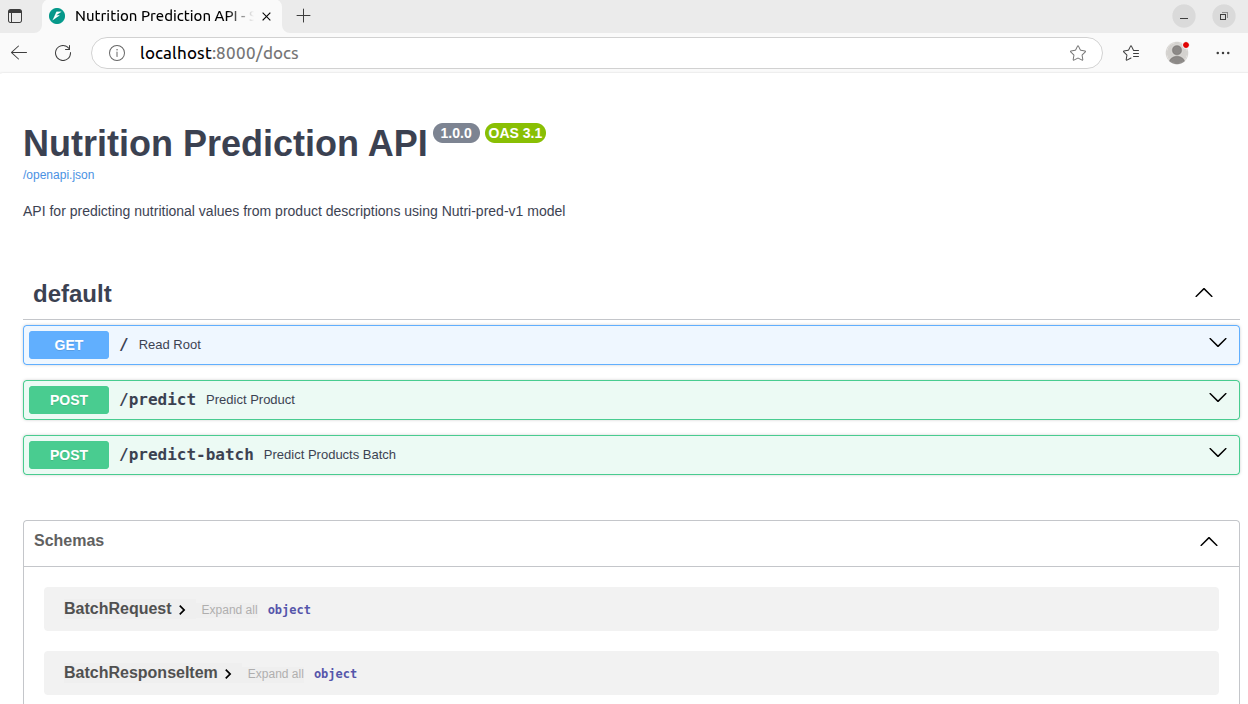
\includegraphics[width=0.98\textwidth]{images/Nutri-pred_fast_API.png}
    \caption{FastAPI endpoint for predicting nutritional values.}
    \label{fig:fastapi-endpoint}
\end{figure}

\vspace{1cm}
The deployment architecture ensures low-latency predictions and supports both local and cloud execution environments. The combination of RESTful access and interactive UI enhances accessibility for developers and non-technical users of this model.

\begin{figure}[H]
    \centering
    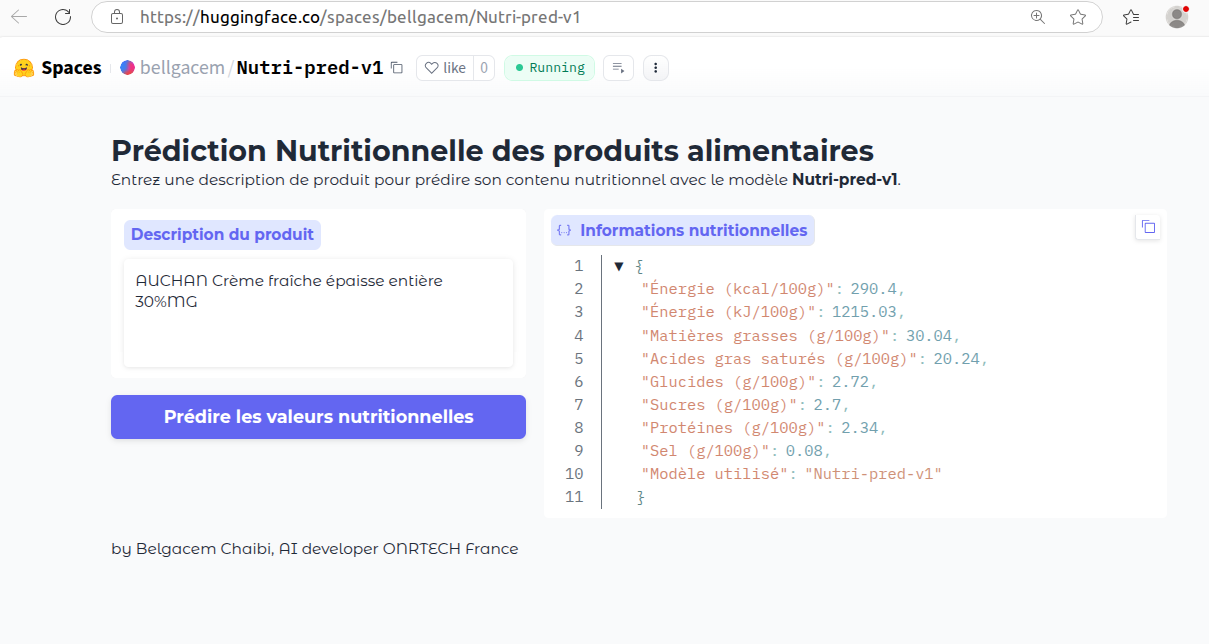
\includegraphics[width=0.99\textwidth]{images/Nutri-pred_Huggingface.png}
    \caption{Gradio interface for Nutri-Pred-v1 hosted on Hugging Face Spaces}
    \label{fig:gradio-ui}
\end{figure}

\newpage
\section{Conclusion}
\par In summary, the Nutri-pred-v1 model represents a significant advancement in our project to predict nutritional values when they are missing
from product descriptions. The KNN algorithm was selected to train
our model for its superior performance in minimizing prediction errors.
This accuracy is crucial for applications in nutritional analysis such as
VitamiNurse, where precise data is essential for informed decision-making.
\par This model is integrated into the data processing pipeline to impute
missing nutritional information. It ensures complete and reliable product
records, which are essential for product evaluation and the recommenda-
tion system described in the following chapter.
\chapter{Implementation of The Data Pipeline}
\section*{Introduction}
\addcontentsline{toc}{section}{Introduction}

This chapter introduces a comprehensive pipeline designed to collect
and process data for our nutrition application. We start by the data
understanding phase, which involves collecting and exploring the data
to identify potential problems. Then, we detail the data preparation
phase, which includes the implementation of an ETL pipeline to clean,
transform, and load the data into a structured format suitable for use by
the recommendation system and the AI assistant. The data is collected
from various European retailers using web scraping techniques that we
will present it with details in a separated section. The collected data is
then cleaned, transformed, and enriched with additional features such as
the Nutri-Score, dietary labels, and other relevant nutritional indicators.
In the final stage, the processed data is embedded and stored in a vector
database to enable efficient semantic search.
\section{Data Understanding}
Following the Business Understanding phase outlined in the first
chapter, we now advance through the remaining CRISP-DM steps.
This section focuses on the Data Understanding phase, which involves
collecting and exploring the data to identify potential problems.

\subsection{Sources}

\par The data used comes mainly from web scraping of a wide variety of
food products in Europe. We scraped data from the websites of major
supermarkets in France, Italy, Germany, and Spain.
The scraped data includes detailed product information and nutritional
values such as calories, carbohydrates, fats, and proteins, as well as
ingredients and allergens.


\subsection{Problems} 
After solving the problem of missing data by building the ML model Nutri-pred-V1, we still face several challenges related to data quality and consistency.
The discarded products are diverse and inconsistent, as they come from
several countries and different distributors.
One major challenge in our project is that product descriptions are
written in different languages, which complicates product matching and
recommendation. As shown in Figure \ref{fig:product_example}, the product description is in
Italian, while other products have descriptions in French, German, or
Spanish. As a result, we need to implement a multilingual approach
to handle these variations effectively. The descriptions show various
inconsistencies, while essential information, including NutriScore and
nutritional labels, is absent from the data.
As a result, an ETL pipeline is required to collect, process, and unify all
products into a consistent database structure.
\begin{figure}[H]
    \centering
    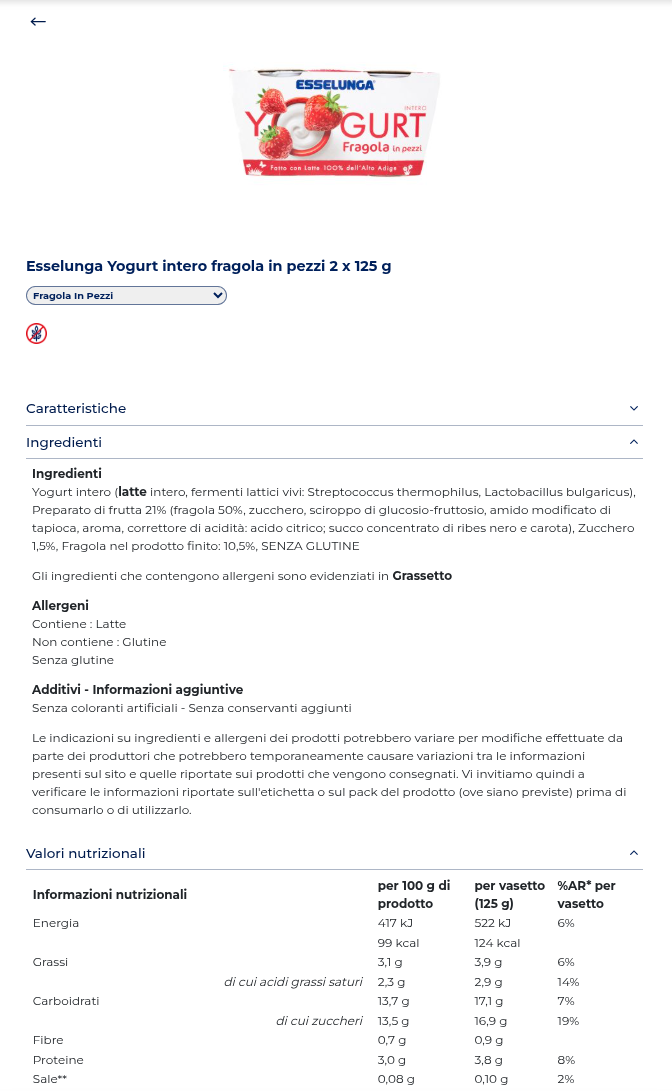
\includegraphics[scale=0.55]{images/product_example.png}
    \caption{An example of a product details page to scrape from the Italian supermarket chain Esselunga} 
    \label{fig:product_example}
\end{figure}


\subsection{Data enrichment}
Another challenge is the nutritional evaluation of each product. It is
impractical to manually assess each product by identifying high-sugar
items for individuals with diabetes or detecting products that do not
contain gluten for people with celiac disease. After the web scraping, the
data pipeline must automatically add pertinent health labels and nutrition
indicators like the Nutri-Score in order to solve this problem. This feature
engineering is a crucial step for enabling efficient product filtering and
delivering personalized recommendations. In parallel, data is enriched
with behavioral data from users’ browsing history on the app, including
products viewed, liked, or disliked, as well as user profiles describing their
dietary preferences, allergies, medical conditions or nutritional goals.

\section{Data Preparation: ETL Pipeline}


The data preparation phase is a crucial step in the CRISP-DM methodology, as it directly impacts the quality and effectiveness of the subsequent
modeling phase. During this phase, we implement an ETL pipeline to
clean, transform, and load the data into a structured format suitable for
use by the recommendation system and the AI assistant. This section
details the technical aspects of the ETL process that was implemented
to collect, process, and integrate products from various European stores,
as well as the tools and methodologies used in this step.

\begin{center}
\begin{figure}[H]
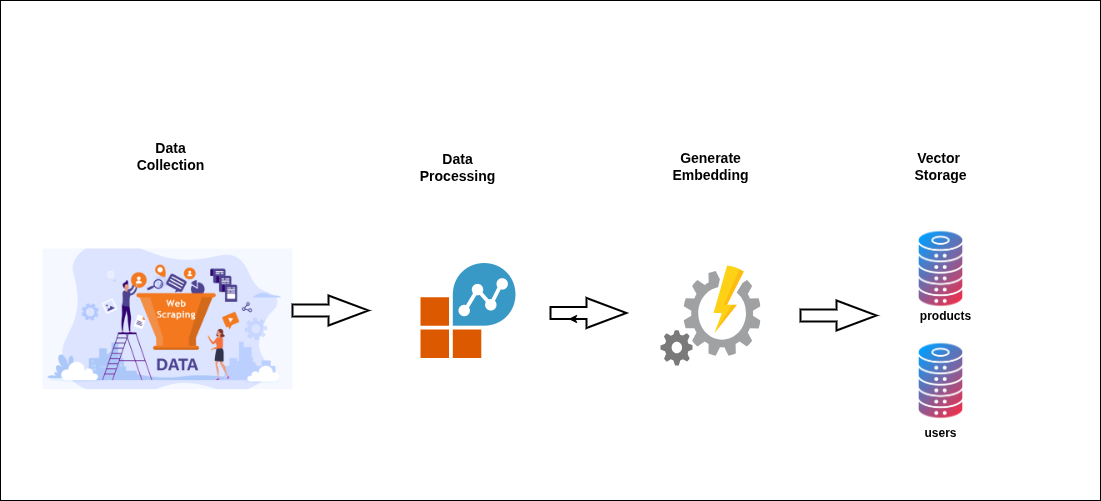
\includegraphics[scale=0.44]{images/workflow__data.png}
\caption{End-to-end data workflow: from web scraping to vector embedding}
\label{fig:data_workflow}
\end{figure}
\end{center}

\subsection{Extract}

\par The starting point in the ETL processing workflow is the data extraction phase. It includes gathering nutritional information, prices, and
descriptions from a range retailer websites using web scraping. Despite the variety of websites available in Europe for scraping, there
are many challenges. The retailers websites have different structures and
categories of products. Selecting the appropriate CSS selectors or HTML
tags for each relevant piece of information is therefore a critical step.

\par The scraped data, as illustrated in Figure \ref{fig:Nutrition_column}, is initially stored in a raw format as JSON files. This raw data serves as the foundation for subsequent processing and transformation steps.
\begin{center}
\begin{figure}[H]
\centering
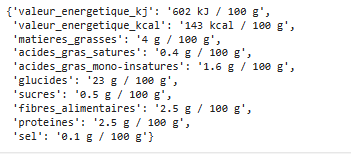
\includegraphics[scale=0.66]{images/nutrition.png}
\caption{Example of a nutrition column before processing} 
\label{fig:Nutrition_column}
\end{figure}
\end{center}

\subsubsection{Web Scraping :}
\par Web scraping is a technique for extracting information from websites by simulating human
browsing behavior. It is particularly useful for gathering large amounts
of data that are not readily available through APIs\cite{2025webscraping}.

\subsubsection{Used Tools in Web Scraping :}
\par We have to relied on a complementary set of tools tailored to the diversity
of data sources and formats encountered.

\begin{itemize}[label=\textbf{-}]
    \item \textbf{Selenium:} was used to automate interactions with dynamic web pages, cookie banners or  AJAX scenarios where data loaded via AJAX is not immediately available in the DOM.
    \item \textbf{BeautifulSoup:}  enabled fast and efficient extraction of information from static HTML content.
    \item \textbf{cURL and Requests :} To interact with REST APIs, cURL and Python’s Requests library allowed for simple HTTP requests, sometimes requiring authentication or specific parameters. 
\end{itemize}

\subsubsection{Web Scraping Process :}

\par In our project, the web scraping process took place in several successive stages as illustrated in Figure \ref{fig:web_scraping_steps} to ensure
efficient information extraction.

\par The first step is the \textbf{page access}. Using Selenium, we automated access
to the various product pages by simulating clicks and navigation between
departments, categories, and subcategories. Then we pass to the \textbf{information extraction}. Once the page loaded, specific information (product name, description, price, images, and storage
instructions) was extracted by analyzing the HTML structure. Particular care was taken to retrieve relevant data, filtering out unnecessary
elements. The final step is \textbf{error handling}. During scraping, error handling mechanisms were implemented to manage potential page blocks, access restrictions, or changes to the page structure. The main challenge we
encountered is anti-bot management. And we can overcome this problem
by using solutions like random delays, proxy rotation, and user agent
switching.

\begin{center}
\begin{figure}[H]
\centering
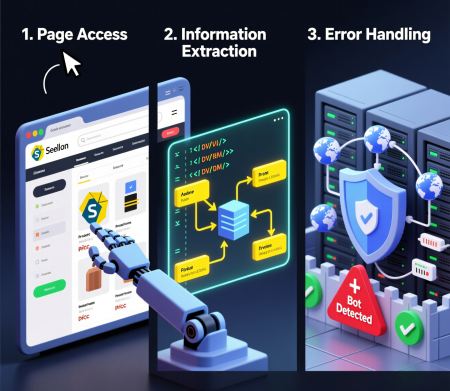
\includegraphics[scale=0.66]{images/web_scraping_steps.png}
\caption{Web Scraping Process Steps} 
\label{fig:web_scraping_steps}
\end{figure}
\end{center}



\subsection{Transform}
After that, The gathered data is cleaned, enriched, and standardized
during the transformation phase to guarantee accuracy and compatibility with VitamiNurse’s requirements.
The scraper provided us with comprehensive product information, including many irrelevant columns. We will extract only the relevant product columns to simplify and focus our
analysis.

\subsubsection{Data Cleaning :}

\par To perform a thorough cleaning, we removed columns
containing products with duplicate EAN codes to eliminate redundancies
and ensure data quality. We also decided to remove columns with
empty nutritional values. Nutritional information was originally located
under the main column "evolutions". We extracted this information and
reorganized it into a separate "nutrition" column, using a dictionary
format.


\subsubsection{Normalization and Transformation :}

\par We had to process the "nutrition" column of our database, since it included detailed nutritional information such as energy, fat, carbohydrates,
protein, and salt for each product. For example, here is an entry from
the "nutrition" column.

\begin{center}
\begin{figure}[H]
    \centering
    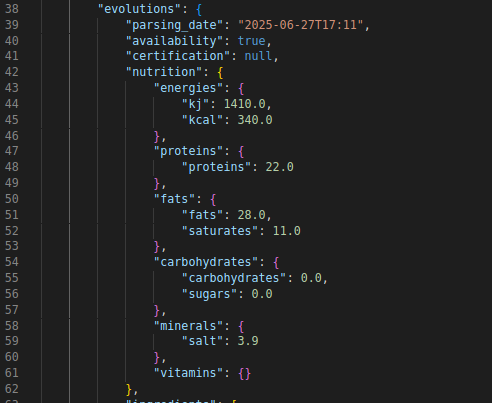
\includegraphics[scale=0.45]{images/transform_nutrition.png}
    \caption{Example of a nutrition column after Normalization and Transformation} 
    \label{fig:Normalization_nutrition}
\end{figure}
\end{center}

\par It was necessary to normalize these data to ensure that they were on
the same scale. Normalization allows feature values to be rescaled so
that they fall within a common range. This is particularly important
for recommendation algorithms, which are sensitive to differences in
magnitude between features. The nutritional values were originally expressed in different units, such as
grams (g), milligrams (mg), and kilocalories (kcal). To enable direct comparison, all nutritional values were normalized to a standard unit per 100 grams (Figure \ref{fig:Normalization_nutrition}). This standardization is essential for the product recommendation process detailed in the next chapter.

\subsubsection{Automated Nutrition Labelling :}

\par After finishing the normalization and transformation of nutritional values, we implemented the first step in feature engineering which is automated nutrition labeling. 
This process involves creating to improve the performance of product evaluation and recommendation algorithms, which requires the construction of a reference dictionary as shown in Figure \ref{fig:nutrition_utils_file}. This reference contains specific keyword lists, such as ingredients that contain gluten, non-vegetarian components, pork-derived ingredients, and substances to avoid during pregnancy. After that we combine all the product titles, ingredients, and categories and check if it matches any specific nutrition keywords from our reference. 
If a match is found, we assign the corresponding label to the product ("gluten-free", "ibs-friendly", "vegetarian", "vegan", "halal", "pregnancy-safe", etc.). This automated labeling process enhances the product metadata, making it easier to filter and recommend products in real-time based on individual dietary needs and preferences.

\begin{center}
\begin{figure}[H]
    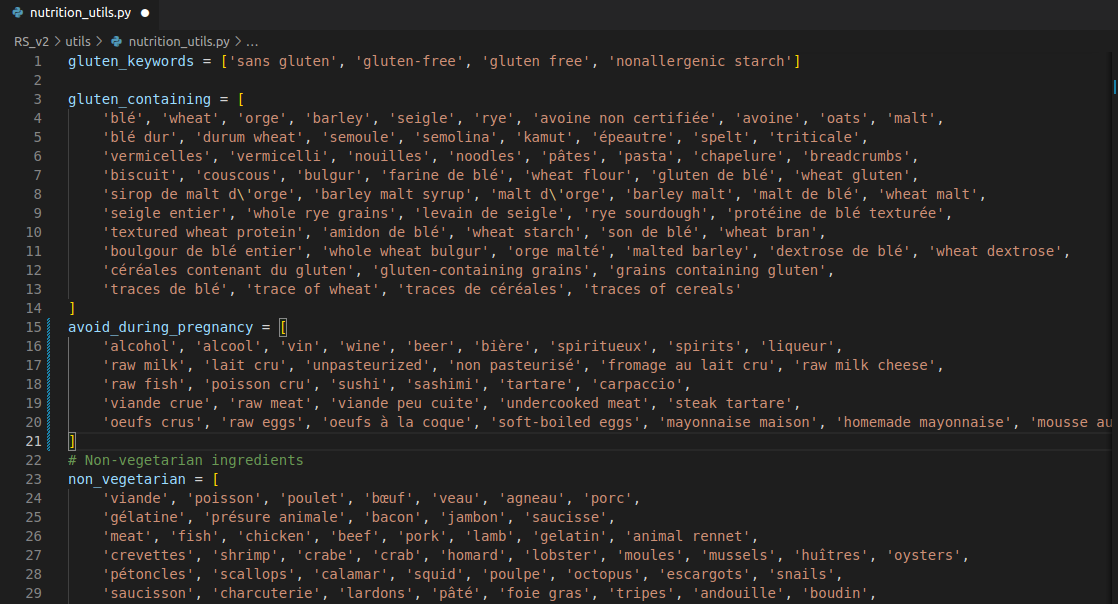
\includegraphics[scale=0.45]{images/nutrition_utils.png}
    \caption{Keywords Dictionary for Automated Nutrition Labelling} 
    \label{fig:nutrition_utils_file}
\end{figure}
\end{center}

\subsubsection{Dietary Labels :}

\par In addition to checking for keywords, we also analyze the nutrition values of each product to assign dietary labels such as "low sugar," "low fat," or "high protein" based on established nutritional guidelines. 
This dual approach of keyword matching and nutritional analysis ensures that each product is accurately labeled according to its health attributes, enhancing the recommendation system's ability to cater to individual dietary needs.

\subsubsection{Nutri-Score Calculation :}

\par The last step in the feature engineering process is the computation and assignment of the
Nutri-Score to each product here. The Nutri-Score is a nutrition label that was first implemented in France
in 2017. It features a five-color scale accompanied by letters from A (most
nutritious) to E (least nutritious)\cite{egnell2022impact}. It is designed to provide consumers
with clear and immediate information about the nutritional quality of
food products. As described by Santé Publique France\cite{santepubliquefrance2025nutriscore}, the system Nutri-Score is adapted to
align with dietary guidelines throughout Europe. In the data pipeline,
we implemented a function that automatically calculates the Nutri-Score
for each product based on its nutritional values. This function follows
the official Nutri-Score algorithm, which considers both negative and
positive nutritional factors to determine the final score.

%\begin{center}
%\begin{figure}[H]
%    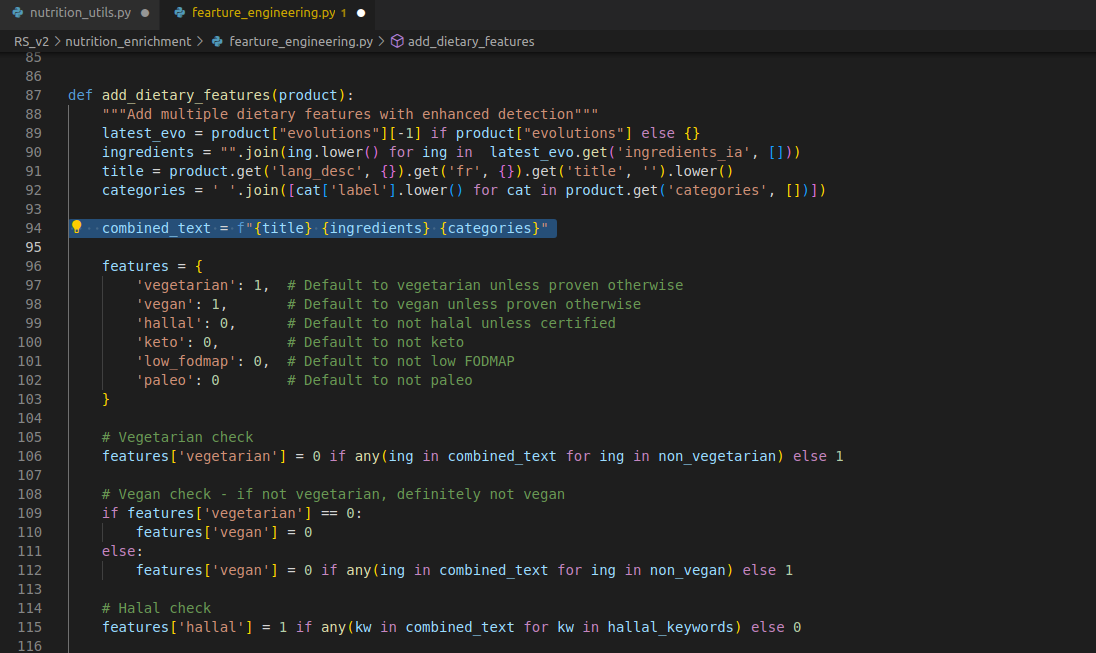
\includegraphics[scale=0.35]{images/feature_engineering.png}
%    \caption{feature engineering} 
%    \label{fig: feature engenieering}
%\end{figure}
%\end{center}


\begin{center}
\begin{figure}[H]
    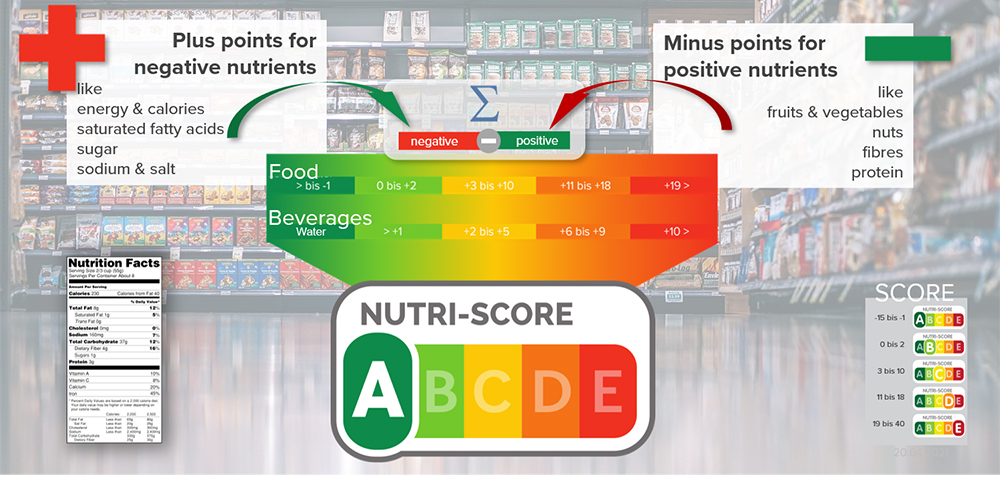
\includegraphics[scale=0.98]{images/nutriscore.jpg}
    \caption{Nutri-Score calculation logic} 
    \label{fig:add_nutriscore}
\end{figure}
\end{center}

\subsection{Load: Data Storage}
After cleaning and transforming the data using an ETL pipeline, the final
phase involves loading the processed information into two complementary
databases to optimize both storage and retrieval.

\subsection{Primary Storage in MongoDB}
As illustrated in Figure\ref{fig:load_data_mongo}, the scraped data are initially stored in MongoDB that serves as the primary database for centralized storage and management. 
This choice guarantees data persistence and reliability, thereby minimizing the risk of data loss while enabling flexible access for subsequent processing stages.


\begin{center}
\begin{figure}[H]
    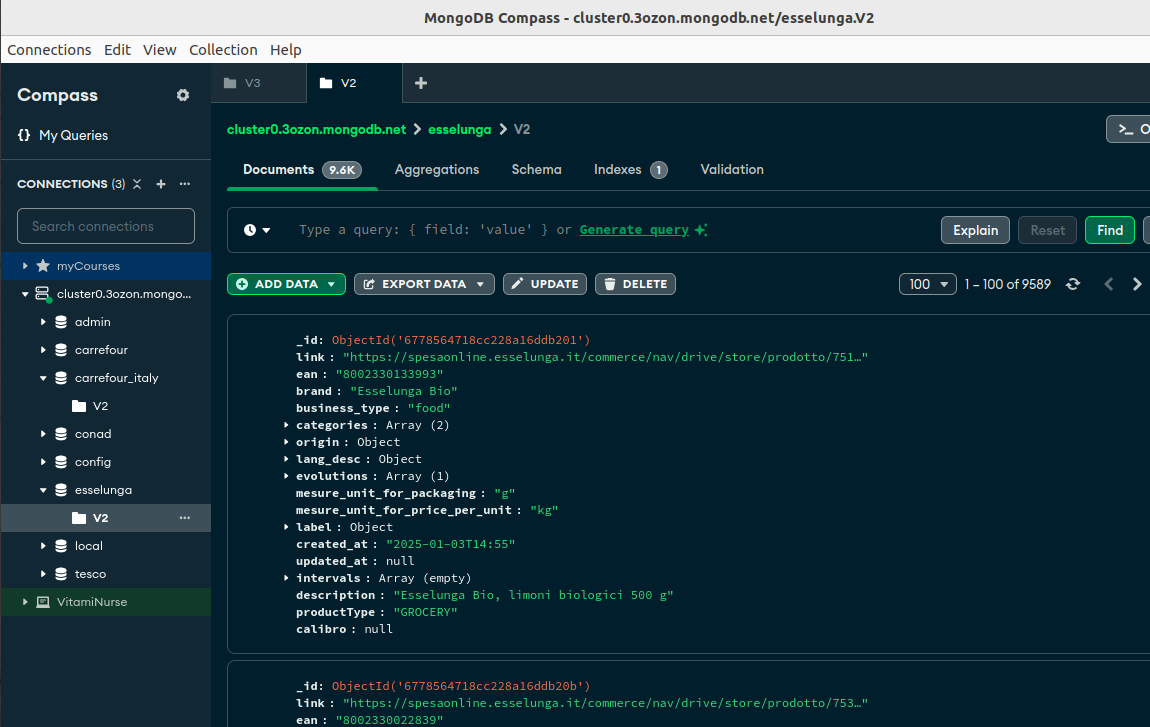
\includegraphics[scale=0.45]{images/load_data.png}
    \caption{Load products for each market in MongoDB} 
    \label{fig:load_data_mongo}
\end{figure}
\end{center}

\subsection{Optimized Vector Store in ChromaDB :}
Following data transformation, a refined copy of the users and products
collections is generated, containing only essential attributes such as
the product name, category, and nutritional information. In order to
optimize retrieval and analysis, this database is then embedded and
stored in ChromaDB. This vector database enables similarity search,
allowing the application to easily access and utilize it for further analysis
or recommendation.


\subsection{Dual-database architecture}
 
This dual-database architecture ensures that the system can efficiently
handle structured queries while also enabling advanced recommendation
and conversational features powered by semantic search.

\par The following tools were employed to facilitate data management, em-
bedding generation, and semantic retrieval:

\begin{itemize}[label=\textbf{-}]
    \item \textbf{MongoDB Atlas}: A cloud-hosted NoSQL database service for the efficient storage and management of structured data, offering scalability and ease of deployment in distributed environments.
    \item \textbf{PyMongo}: A robust Python library that enables seamless programmatic interaction with MongoDB instances, supporting operations such as data insertion, querying, and updates.
    \item \textbf{MongoDB Compass}: An intuitive graphical user interface tool for exploring MongoDB collections and visualizing data.
    \item \textbf{ChromaDB}: An open-source vector database optimized for high-dimensional embeddings and enabling efficient similarity searches, particularly suited for semantic querying tasks.
    \item \textbf{SentenceTransformers}: A Python-based library that uses transformer models to generate dense vector representations (embeddings) from textual input.
\end{itemize}






\section*{Conclusion}
In conclusion, we can provide a robust foundation for ingesting and processing data from multiple platforms by building a robust data pipeline.
This pipeline ensures that the data is clean, standardized, and enriched
with relevant features, making it suitable for powering the recommendation system and AI assistant. Furthermore, to optimize semantic search
and enable real-time personalized recommendations, we implemented a vector database for efficient data storage and retrieval. To ensure data
completeness and support accurate recommendations, a machine learning model is also trained to predict missing values. 
The next chapters will focus on the recommendation system and the AI assistant, detailing how they leverage this well-prepared data to deliver personalized nutrition advice and product suggestions to users.
\chapter{Development of Recommendation
System}
\section*{Introduction}
This chapter presents the architectural design, implementation methodology, and empirical evaluation of the hybrid recommendation system
developed for the VitamiNurse mobile application. The system employs
a multi-modal architecture that integrates collaborative filtering, contentbased filtering, and real-time behavioral analytics to deliver personalized
nutritional recommendations aligned with users’ health profiles, dietary
restrictions, and preferences.
The chapter begins with an analysis of vector databases as foundational
infrastructure for semantic retrieval, including a detailed discussion of approximate nearest neighbor (ANN) search and the Hierarchical Navigable
Small World (HNSW) algorithm. Subsequent sections detail the system’s
hybrid architecture, algorithmic components, embedding strategies, and
deployment pipeline.

\section{Vector Databases and Semantic Retrieval}
Vector databases serve as the backbone of modern content-based recommendation systems by enabling efficient similarity search in highdimensional embedding spaces.
In VitamiNurse, they facilitate the semantic matching of user health
profiles with nutritional products based on dietary needs, allergies, and
wellness goals.
\subsection{Fundamentals of Vector Databases}
Vector databases store and index dense numerical representations (embeddings) of data objects, allowing retrieval based on semantic similarity
rather than exact keyword matches [14]. Each item is mapped to a point
in a continuous vector space, where proximity reflects conceptual relatedness. Similarity is typically measured using cosine distance or Euclidean
norms, enabling applications such as semantic search, recommendation,
and clustering.

\begin{figure}[H]
\centering
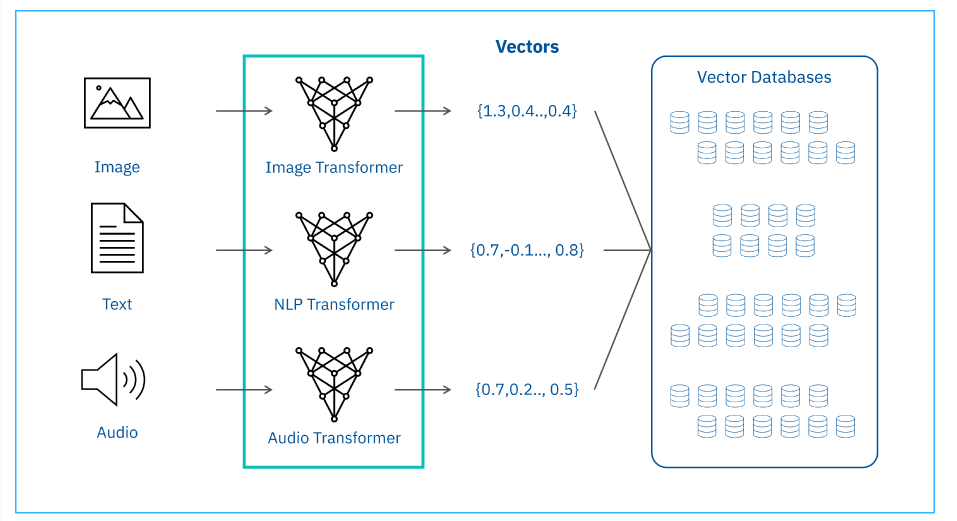
\includegraphics[scale=0.45]{images/vectorDB.png}
\caption{Embedding representation in a vector database}
\label{fig:vectorDB}
\end{figure}

\subsection{Approximate Nearest Neighbor Search}
Based on comparing a query vector against all stored vectors, exact
similarity search becomes computationally prohibitive as dataset size
grows particularly in high-dimensional spaces due to the “curse of dimensionality” [15].
Approximate Nearest Neighbor (ANN) algorithms address this limitation
by sacrificing marginal accuracy for substantial gains in speed and memory
efficiency. These methods construct specialized index structures (e.g.,
trees, hash tables, or graphs) that enable sublinear-time retrieval of
near-optimal neighbors.
\subsection{HNSW Algorithm}
Among ANN techniques, the Hierarchical Navigable Small World (HNSW)
algorithm has emerged as a state-of-the-art solution for large-scale similarity search [16]. HNSW organizes vectors into a multi-layer graph: upper
layers contain sparse, long-range connections for rapid coarse navigation,
while lower layers provide dense, local links for fine-grained refinement.
Search begins at the top layer and descends iteratively, achieving logarithmic time complexity with high recall. This balance of speed and
accuracy makes HNSW ideal for real-time recommendation systems.
\subsection{Selection of ChromaDB}
ChromaDB was selected as the vector database for VitamiNurse due to
its native support for HNSW indexing and native support for HNSW
indexing under an open-source license [17]. A critical feature is its ability
to update the vector index dynamically without full retraining, which is
essential for the system’s daily synchronization of product metadata from
external retailers. Additionally, ChromaDB supports metadata filtering
alongside vector search, allowing post-retrieval enforcement of health
constraints such as excluding gluten-containing products for celiac users.

\begin{figure}[H]
    \centering
    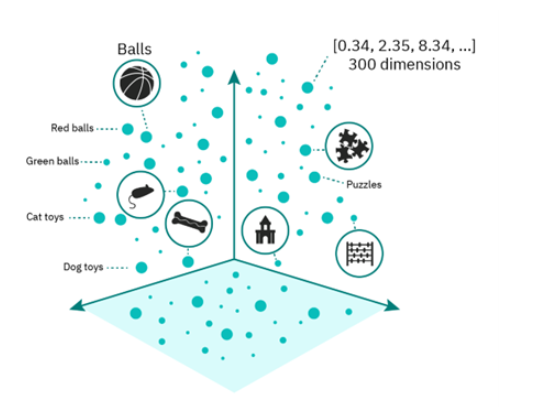
\includegraphics[scale=0.66]{images/chroma_space.png}
    \caption{Vector search mechanism in ChromaDB using HNSW}
    \label{fig:vector_search}
\end{figure}

\subsection{Vector Search Versus Traditional Keyword Search}
Traditional search relies on discrete tokens and exact matching, limiting
its ability to generalize across semantically related terms. In contrast,
vector search retrieves items based on embedding proximity. For example,
a query for “dark chocolate” may return “organic cacao snacks” if their
embeddings are close, even in the absence of shared keywords. This
capability is essential for delivering nutritionally appropriate alternatives
that align with user health objectives.

\subsection{Embedding Generation}
Dense vector representations are produced using transformer-based sentence encoders. These models map textual descriptions of products and
user profiles into fixed-dimensional spaces where semantic relationships
are preserved geometrically. Efficient indexing and retrieval of these
embeddings are enabled by ANN algorithms such as HNSW, ensuring
scalability without compromising relevance.

\section{System Architecture}
VitamiNurse employs a \textbf{modular hybrid architecture}, separating
collaborative and content-based filtering into specialized components:

\item \textbf{CLightFM (Pure Collaborative):} I Captures long-term user preferences via matrix factorization, trained only on interaction data to avoid metadata-induced noise.
\item \textbf{ChromaDB (Content-Based):}  Handles real-time product similarity using HNSW, enabling rapid updates without model retraining.
\subsection{Hybrid Architecture Design}
VitamiNurse implements a hybrid recommendation system that combines
offline collaborative filtering (CF) with real-time, nutrition-aware contentbased filtering (CBF). The collaborative component uses LightFM, trained
nightly at 00:00 on user interaction data (views, likes, dislikes) to capture
long-term preferences without metadata bias. In parallel, a contentbased pathway leverages ChromaDB with HNSW indexing to perform
low-latency similarity searches over product embeddings generated by
the all-MiniLM-L6-v2 model.

When a user scans a product, the system retrieves semantically similar
items and re-ranks them according to the nutrition profile of the user.
This profile is continuously updated in real-time by its interactions with
the Nutrition AI Assistant.

Final recommendations are produced via a weighted ensemble (60\%
content-based, 40\% collaborative), prioritizing immediate nutritional
relevance while retaining historical preference signals. The architecture is
organized into four layers—data ingestion, embedding generation, hybrid
recommendation, and API serving—enabling scalable, responsive, and
health-conscious personalization.

\begin{figure}[H]
\centering
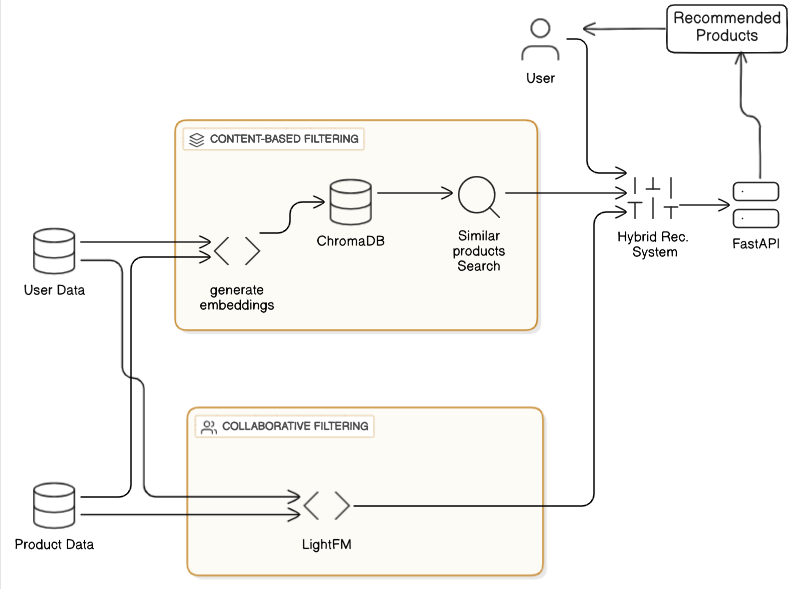
\includegraphics[scale=0.55]{images/RS_Arch.png}
\caption{Overall architecture of the recommendation system}
\label{fig:Recommendation_Sequence_Diagram}
\end{figure}

\subsection{Hybrid System with Decoupled Components}
Although the LightFM framework supports two principal modes : \textbf{pure
collaborative filtering} and \textbf{hybrid filtering}, we chose to employ only
the pure collaborative model for VitamiNurse’s recommendation system.
The system integrates collaborative filtering (CF) and content-based
filtering (CBF) through a weighted ensemble approach. These approaches
are combined in a hybrid recommender, which assigns weighted scores
(60\% content-based powered by ChromaDB, 40\% collaborative with
LightFM) to rank recommendations. This decision was made after
extensive evaluation and careful alignment with the platform’s realtime infrastructure requirements. The selected approach offers greater
scalability and modularity, particularly given the dynamic nature of our
product catalog and metadata. The following subsections outline the key
architectural and empirical factors that guided this choice.
\\
\textbf{Why Not LightFM Hybrid?}
\\
While hybrid models are often assumed to enhance performance by
incorporating additional features, we avoided LightFM’s hybrid mode for
the following reasons:

\paragraph{1) Real-time Product Updates and Scalability Requirements}

VitamiNurse’s product database synchronizes daily with external retail inventories, meaning metadata (e.g., categories, availability) can change frequently. A hybrid LightFM model would require retraining whenever item features update, introducing latency and scalability challenges. In contrast, our content-based filtering module (powered by ChromaDB with HNSW-based approximate nearest neighbor search) dynamically adapts to metadata changes without retraining, making it better suited for real-time updates [18].

ChromaDB’s vector infrastructure is optimized for large-scale similarity
search, supporting millions of product embeddings with efficient retrieval.
This eliminates the need to encode metadata directly into LightFM, as
the content-based component handles this asynchronously and with lower computational overhead.
\paragraph{2) Benchmark Evidence

Pure LightFM Outperforms Hybrid LightFM}
Empirical studies consistently demonstrate that LightFM’s pure collaborative
model achieves superior performance compared to its hybrid counterpart:

\begin{itemize}
\item \textbf{MovieLens 100k Benchmark:} [19] evaluated LightFM on the
MovieLens dataset, showing that the pure model outperformed the
hybrid variant in precision@K and recall@K across cutoffs (K=5, 10,
20). The hybrid model not only underperformed but also failed to
surpass simpler baselines like ItemKNN in some metrics as illustrated
in Figure 4.4.
\item \textbf{Feature Noise:} The inclusion of item features degraded performance, likely due to redundant or poorly weighted metadata. [19]
found that the hybrid model’s precision\@5 was worse than graphbased baselines like P3\α and RP3\β.
\item \textbf{Community Reports:} GitHub issues and user reports corroborate
these findings, with cases where shuffled or irrelevant item features
further reduced model accuracy [20].
\end{itemize}

\paragraph{3) Computational Efficiency}

Pure collaborative filtering requires fewer
computational resources during training and inference. Benchmarks on
the Movielens 20M dataset show that LightFM’s inference speed scales
linearly with latent factor dimensionality, but hybrid models introduce
additional overhead from feature processing.

This decoupling aligns with industry best practices, where hybrid \textit{systems} (not hybrid \textit{models}) often deliver more robust performance. This
architecture ensures scalability while maintaining interpretability and
efficiency.
\subsection{Dynamic Data Update and Sync Architecture}
The VitamiNurse system operates through a robust, modular data
pipeline designed for real-time responsiveness and adaptability to both
user behavior and product catalog changes:
\begin{enumerate}
\item \textbf{ Real-time Interaction Tracking:} 

User activities, such as viewing, liking, and disliking products, are continuously monitored and
recorded. These interactions directly inform the recommendation
engine, ensuring up-to-date and personalized suggestions.
\item \textbf{Dynamic Profile Synchronization:} 

Upon any profile change
(e.g., allergy updates, changed health conditions, pregnancy status),
the system triggers immediate re-embedding of the user’s profile
vector within ChromaDB. This ensures atomic, consistent updates
that instantly reflect in recommendations, without disrupting the
user’s session.
\item \textbf{ Automated Product Ingestion and Embedding:} 

The product
catalog is synchronized daily with partner retailers. New or modified
products are automatically detected, vectorized through semantic
embedding, and integrated into the recommendation graph using a
CDC (Change Data Capture) pipeline.

\item \textbf{Daily Model Retraining:}

To adapt to evolving user preferences
and product changes, the LightFM recommendation model is retrained every 24 hours (scheduled at 00:00 UTC). This ensures
continuous learning and optimal recommendation quality.
\end{enumerate}

\section{Content-based filtering}
The content-based (CB) recommendation module in VitamiNurse is
designed to provide personalized nutritional product suggestions by leveraging semantic similarity between user profiles and product characteristics.
This is achieved through dense vector embeddings stored in ChromaDB
and computed using a lightweight sentence-transformer model.

\subsection{Embedding Model Evaluation}


\begin{table}[h!]
\centering
\resizebox{0.9\textwidth}{!}{%
\begin{tabular}{@{}lccccc@{}}
\toprule
\textbf{Model Name} & \textbf{Sent. Emb.} & \textbf{Sem. Search} & \textbf{Avg. Perf.} & \textbf{Speed} & \textbf{Size} \\
\midrule
\textbf{all-mpnet-base-v2} & \textbf{69.57} & \textbf{57.02} & \textbf{63.30} & \textbf{2800} & 420 MB \\
multi-qa-mpnet-base-dot-v1 & 66.76 & 57.60 & 62.18 & 2800 & 420 MB \\
all-distilroberta-v1 & 68.73 & 50.94 & 59.84 & 4000 & 290 MB \\
all-MiniLM-L12-v2 & 68.70 & 50.82 & 59.76 & 7500 & 120 MB \\
multi-qa-distilbert-cos-v1 & 65.98 & 52.83 & 59.41 & 4000 & 250 MB \\
\textbf{all-MiniLM-L6-v2} & \textbf{68.06} & \textbf{49.54} & \textbf{58.80} & \textbf{14200} & 80 MB \\
multi-qa-MiniLM-L6-cos-v1 & 64.33 & 51.83 & 58.08 & 14200 & 80 MB \\
paraphrase-multilingual-mpnet-base-v2 & 65.83 & 41.68 & 53.75 & 2500 & 970 MB \\
paraphrase-albert-small-v2 & 64.46 & 40.04 & 52.25 & 5000 & 43 MB \\
paraphrase-multilingual-MiniLM-L12-v2 & 64.25 & 39.19 & 51.72 & 7500 & 420 MB \\
paraphrase-MiniLM-L3-v2 & 62.29 & 39.19 & 50.74 & 19000 & 61 MB \\
distiluse-base-multilingual-cased-v1 & 61.30 & 29.87 & 45.59 & 4000 & 480 MB \\
distiluse-base-multilingual-cased-v2 & 60.18 & 27.35 & 43.77 & 4000 & 480 MB \\
\bottomrule
\end{tabular}
}
\caption{Performance comparison of SentenceTransformer models. Speed is measured as average sentences processed per second.}
\label{tab:models}
\end{table}
Speed is measured as average
sentences processed per second.
\\
 The \textit{SentenceTransformers} library offers a range of models evaluated for
their performance in generating sentence embeddings and conducting
semantic search, based on two key criteria: the quality of cross-sentence
representations across 14 datasets and the effectiveness in semantic search
tasks on 6 datasets.
The \textbf{all-*} models, trained on an extensive corpus of over one billion text
pairs, are designed as general-purpose models, with \textit{all-mpnet-base-v2} delivering the highest overall quality and \textit{all-MiniLM-L6-v2} providing comparable quality at approximately five times the speed, making it an
efficient choice for various applications [21].


\subsection{Embedding Model Selection}
The system employs the all-MiniLM-L6-v2 model for generating embeddings, which offers several advantages over alternatives. By being
fine-tuned on over 1 billion text pairs, the all-MiniLM-L6-v2 excels in
semantic similarity tasks. Despite its smaller size, it achieves 93\% the
accuracy of larger models such as BERT-base models.
This sentence transformer model is an excellent choice for VitamiNurse
recommendation system, as it produces 384-dimensional embeddings that
effectively capture subtle relationships within the data. [22] Furthermore,
its compact architecture, with only 33.4 million parameters, enables
efficient CPU-only inference, and multilingual support enables global
applicability. The model’s balance of speed, accuracy, and resource
efficiency makes it ideal for real-time recommendation scenarios in the
VitamiNurse application.
\subsection{CB Recommendation Process}

\paragraph{Query Construction}
\\
The CB system operates based on two possible inputs: the \textbf{user identifier}
and an optional \textbf{scanned product identifier} (EAN code). When a
user scans a product, the system retrieves metadata associated with that
item such as product name, brand, categories, and nutrition information.
Simultaneously, it extracts the user’s profile information, which includes
dietary preferences, pregnancy status, and medical conditions like diabetes
or hypertension.\\
These two sources of information are merged to create a descriptive
query that captures both the scanned product’s features and the user’s
health-related needs.
\paragraph{Search and Recommendation}

The query is then embedded into a vector using the selected embedding
model and used to perform a semantic search in the product database.
The search returns a list of nutritionally and semantically similar products.
In cases where no product is scanned, the recommendation relies entirely
on the user’s profile to infer their preferences and health requirements.
Based on this information, it generates a personalized query, which is
then used to display tailored recommendations on the home page.

\paragraph{Recommendation Score}

Each recommended product is assigned a relevance score based on semantic proximity. This score is further refined by applying domain specific
nutritional rules by boosting products with better Nutri-Scores. The
system also applies post-filtering to strictly enforce compatibility with
medical conditions or dietary restrictions. For instance, a user with celiac
disease will never be recommended a product that contains gluten, even
if it is semantically similar.
\paragraph{CB Recommendation Workflow}

The content based recommendation workflow follows a structured process
in order to offer a personalized and health-aware user experience, as
illustrated in the following diagram. It begins by metadata gathering
and query construction. Queries are embedded into vectors using the allMiniLM-L6-v2 model for semantic search against the product database.
The system then selects and returns recommendations aligned with user
preferences and nutritional needs.\\
This design ensures that the products delivered by the content based
recommendation system are not only contextually relevant but also
aligned with the unique nutritional profile of each user of VitamiNurse
app.
\section{Collaborative Filtering}
Collaborative filtering in \textit{VitamiNurse} leverages the \textbf{LightFM model},
which combines matrix factorization and metadata-aware learning.
\subsection{Overview}
Collaborative filtering (CF) is a widely used recommender system technique that predicts user preferences by leveraging the collective behavior
of similar users or items. As defined by IBM, CF operates on the principle
that users with shared interests in the past will likely agree in the future, making recommendations based on patterns identified in user-item
interaction matrices [23].

\begin{figure}[H]
\centering
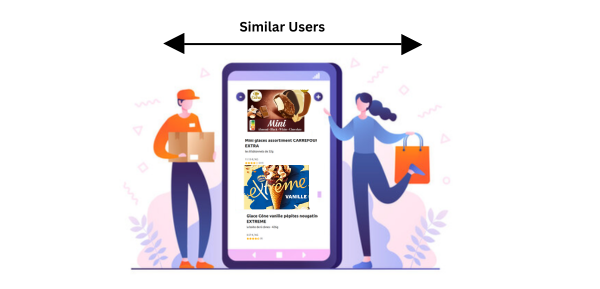
\includegraphics[scale=0.85]{images/collaborative_filtering.png}
\caption{Collaborative filtering logic}
\label{fig:cf_workflow}
\end{figure}

\subsection{LightFM’s Collaborative Filtering Approach
}
LightFM implements a hybrid matrix factorization model rather than
traditional memory-based (neighborhood) collaborative filtering. Unlike
user/item-neighborhood methods that rely on cosine similarity or Pearson
correlation [23], LightFM learns latent embeddings using Weighted Matrix
Factorization (WMF) or Bayesian Personalized Ranking (BPR) loss. This
approach is scalable and well-suited for sparse datasets, making it ideal
for recommendation systems like VitamiNurse.

\subsection{ Creation of the Interaction Matrix}
VitamiNurse incorporates multiple types of user feedback, each assigned
specific weights to reflect varying degrees of preference:

Table 4.2: Interaction types and corresponding weight values
\\
\\
manque le tableau


\\

\subsection{Loss Functions in LightFM}
The LightFM library supports multiple loss functions tailored to different
recommendation scenarios:
\begin{itemize}
\item \textbf{WARP} (Weighted Approximate-Rank Pairwise): Optimized for
ranking tasks with implicit feedback (clicks). It focuses on positive signals and is effective for top-N recommendations but does not
handle negative feedback well.
\item \textbf{BPR} (Bayesian Personalized Ranking): Designed for personalized
item ranking through pairwise comparisons. It ranks preferred items
higher than less preferred or irrelevant ones, accommodating nuanced
feedback.
\item \textbf{Logistic}: Used for probabilistic modeling, typically with explicit
feedback (ratings)
\end{itemize}

\subsection{ Selection of Loss Function}
The selection of an appropriate loss function is critical in recommendation
systems, as it determines how user-item interactions are modeled during
the training process. Collaborative filtering leverages implicit feedback
(likes, views, dislikes) weighted as shown in Table 4.2 to inform this
process.

Our collaborative module cannot use WARP loss because it fails to model
explicit dislikes (-1.0). Instead, \textbf{Bayesian Personalized Ranking}
(BPR) was chosen because it optimizes pairwise comparisons, explicitly
ranking liked items higher than visited or disliked ones while leveraging
both positive and negative signals. This approach better aligns with
VitamiNurse’s goal of learning from complex user interactions while
maintaining scalability on sparse datasets.

\section{Benchmarking the Recommendation System:
Exact vs. ANN (HNSW) Search}

To ensure both scalability and precision, we benchmarked two vector
search modes available in ChromaDB: the default exact search and the
HNSW-enabled Approximate Nearest Neighbor (ANN) search.
\subsection{Theoretical Comparison}
Exact search is ChromaDB’s default method . It performs exhaustive
comparisons between the query vector and all stored vectors using cosine
similarity, ensuring maximum precision. However, this method can
become computationally expensive as the dataset grows.
As we have seen, HNSW search is an approximate nearest neighbor
(ANN) technique that is frequently adopted in large-scale recommender
systems. It constructs a navigable graph index that accelerates retrieval.
Although it introduces a slight drop in precision, it significantly enhances
speed and scalability.
The following table summarizes the key differences between the two
modes:
\\

Table 4.3: Key Differences: Default vs. HNSW Search
\\
\\

\subsection{Experimental Results and Scalability Implications}
We benchmarked 20,000 recommendation requests using ChromaDB with
23,000 products indexed. Both modes—Exact (port 8000) and HNSW
(port 8001) returned valid top-10 results for each request with a 100\%
success rate.

\\
Table 4.4: Benchmark Results for Recommendation Modes

\\
Results demonstrate that \textbf{HNSW} significantly outperforms exact search
in terms of speed (from 187.4ms to 178.08ms), even with only 23,000
products. As VitamiNurse scales to hundreds of thousands or even
millions of products across Europe and the US, the cost of exact search
will become increasingly prohibitive.
HNSW, by contrast, offers scalable performance with near-equivalent
accuracy, making it the preferred choice for large-scale deployments in
real-time production environments.
Results demonstrate that \textbf{HNSW} significantly outperforms \textbf{exact
search} on speed while maintaining high relevance in practical use cases.
It is now the preferred mode for large-scale deployments in VitamiNurse.

\section{ Deployment}
\subsection{FastAPI Deployment}
To facilitate real-time access to personalized nutritional recommendations
within the \textit{VitamiNurse} mobile application, the recommendation engine
is exposed through a RESTful API developed using a private \textbf{FastAPI}
service. We chose FastAPI for its performance, asynchronous capabilities,
and automatic data validation using Pydantic.

Our API provides a single endpoint, \/recommend, which receives structured input from the app (user ID, scanned EAN,limit, recommendation\_type) and returns tailored food item suggestions in JSON format.

\subsection{ Multi-Modal Recommendation Deployment}
The API supports three recommendation modes selectable via a recommendation type parameter:
\begin{enumerate}
\item Collaborative filtering
\item Content-based filtering
\item  Hybrid approach
\end{enumerate}
This internal service ensures fast, reliable, and scalable communication
between the app and the recommendation system. Although fully documented through FastAPI’s auto-generated Swagger UI, the API will be
accessed exclusively by the mobile app and the development team for
testing.

\begin{figure}[H]
\centering
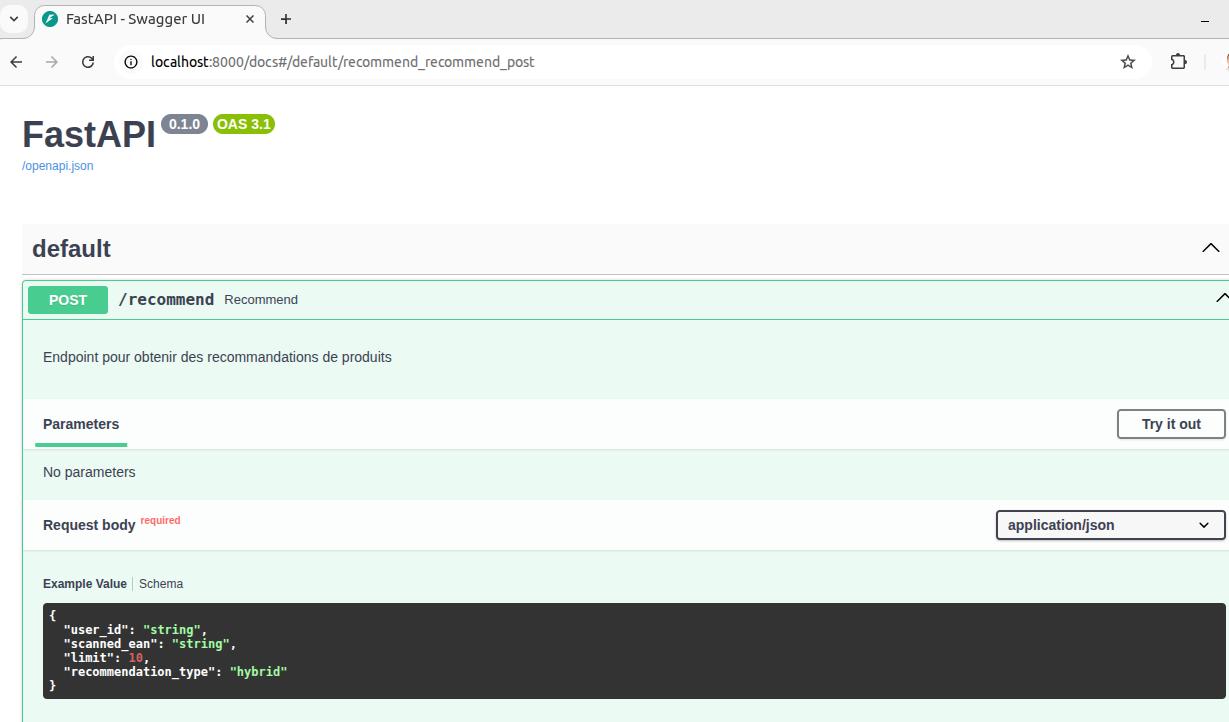
\includegraphics[scale=0.35]{images/swaggerFastAPI.png}
\caption{Swagger UI for the internal Recommendation API}
\label{fig:swagger_UI}
\end{figure}













\paragraph{2. Empirical Performance}
Benchmarking on MovieLens 100k \cite{shu2023lightfm} shows:
\item Pure LightFM outperforms hybrid LightFM in precision@K and recall@K.
    \item Item features often introduce noise, degrading performance.
    \item Hybrid LightFM underperforms simpler baselines like ItemKNN and RP3$\beta$.

\begin{figure}[H]
    \centering
    \begin{minipage}{0.48\textwidth}
        \centering
        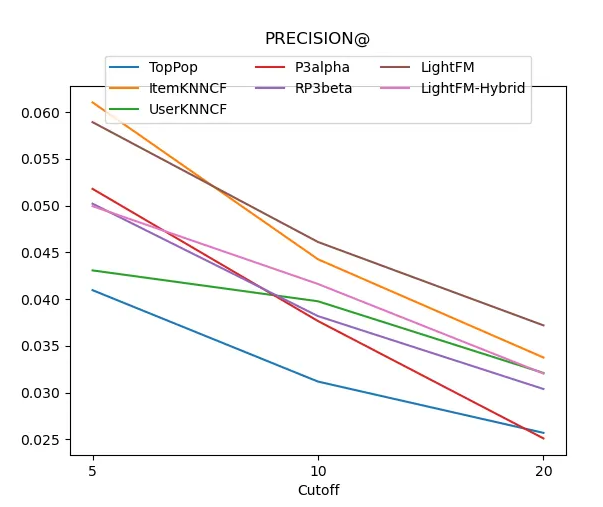
\includegraphics[width=\linewidth]{images/precision_plot.png}
        \caption{Precision@K comparison}
        \label{fig:precision}
    \end{minipage}\hfill
    \begin{minipage}{0.48\textwidth}
        \centering
        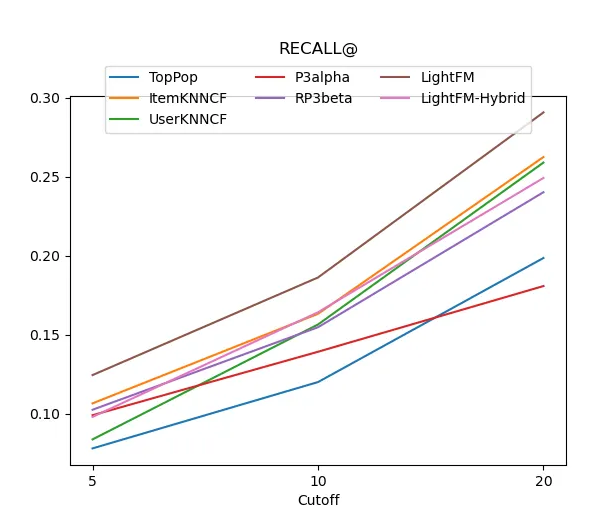
\includegraphics[width=\linewidth]{images/recall_plot.png}
        \caption{Recall@K comparison}
        \label{fig:recall}
    \end{minipage}
\end{figure}

\paragraph{3. Computational Efficiency}
Pure CF reduces training/inference overhead, enabling faster daily retraining and lower operational costs.

This decoupled approach aligns with industry best practices: **hybrid systems** (not hybrid models) offer greater flexibility and maintainability.

\subsection{Dynamic Data Pipeline}
The system supports continuous adaptation through:
\begin{enumerate}
    \item \textbf{Real-time interaction logging}
    \item \textbf{Profile-triggered re-embedding} (e.g., allergy updates)
    \item \textbf{CDC-based product ingestion} (Change Data Capture from retailers)
    \item \textbf{Daily LightFM retraining} (scheduled at 00:00 UTC)
\end{enumerate}

\section{Content-Based Filtering Module}
\subsection{Semantic Personalization via Embeddings}
The CBF module generates recommendations by computing semantic similarity between:
\item User profile (dietary preferences, health conditions)
    \item Product metadata (name, category, nutrition facts, allergens)

\begin{figure}[H]
\centering
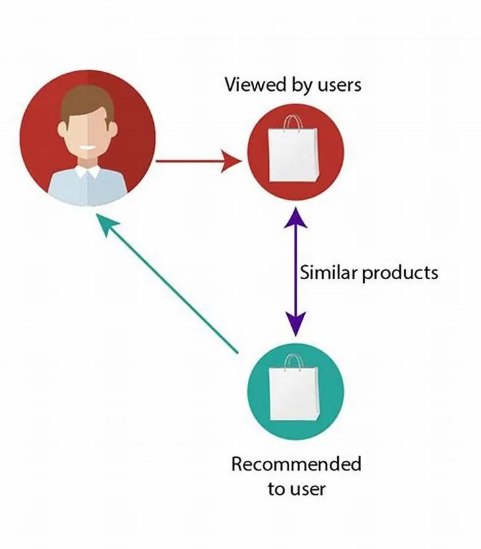
\includegraphics[scale=0.35]{images/cb_filtering_logic.png}
\caption{Logic of content-based filtering in VitamiNurse}
\label{fig:CB_filtering_logic}
\end{figure}

\subsection{Embedding Model Selection}
We evaluated multiple SentenceTransformer models (Table~\ref{tab:models}). \texttt{all-MiniLM-L6-v2} was selected for its optimal trade-off:

\begin{table}[H]
\centering
\caption{Performance comparison of SentenceTransformer models}
\label{tab:models}
\resizebox{0.9\textwidth}{!}{%
\begin{tabular}{@{}lccccc@{}}
\toprule
\textbf{Model} & \textbf{Sent. Emb.} & \textbf{Sem. Search} & \textbf{Avg. Perf.} & \textbf{Speed (sent/s)} & \textbf{Size} \\
\midrule
all-mpnet-base-v2 & 69.57 & 57.02 & 63.30 & 2800 & 420 MB \\
\textbf{all-MiniLM-L6-v2} & \textbf{68.06} & \textbf{49.54} & \textbf{58.80} & \textbf{14200} & \textbf{80 MB} \\
\bottomrule
\end{tabular}%
}
\end{table}

It achieves 93\% of BERT-base accuracy with 5× faster inference and minimal memory footprint—ideal for mobile backend deployment.

\subsection{Data Ingestion into ChromaDB}
Product metadata is embedded using \texttt{all-MiniLM-L6-v2} and loaded into ChromaDB with HNSW indexing. The compact 384-dimensional vectors enable efficient CPU-based inference and multilingual support.

\begin{figure}[H]
\centering
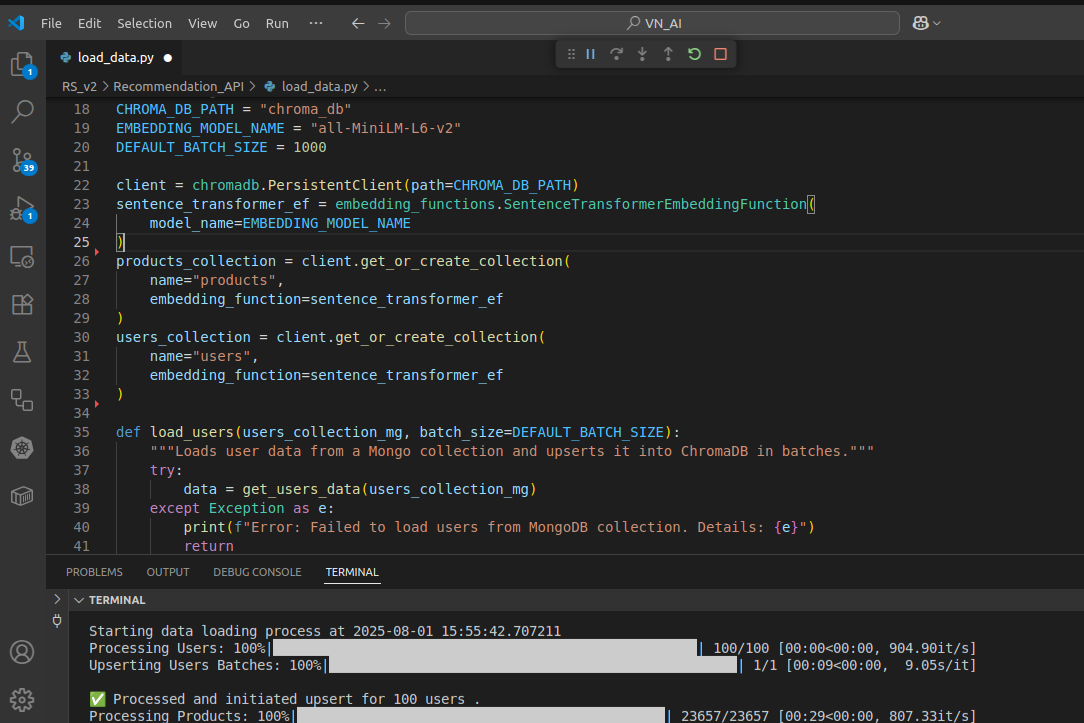
\includegraphics[scale=0.39]{images/load_data__0.png}
\caption{Data loading pipeline into ChromaDB}
\label{fig:load_data_chroma}
\end{figure}

\subsection{Recommendation Workflow}
\subsubsection{Query Construction}
Inputs:
\item User ID (mandatory)
    \item Scanned product EAN (optional)
The system fuses user health profile and product metadata into a single semantic query.

\subsubsection{Semantic Search and Ranking}
The query is embedded and used to retrieve top-\(k\) similar products via HNSW search.

\subsubsection{Post-Processing and Scoring}
Results are:
\item Re-ranked by Nutri-Score (healthier products boosted)
    \item Hard-filtered for medical/dietary constraints (e.g., no gluten for celiac users)

\begin{figure}[H]
\centering
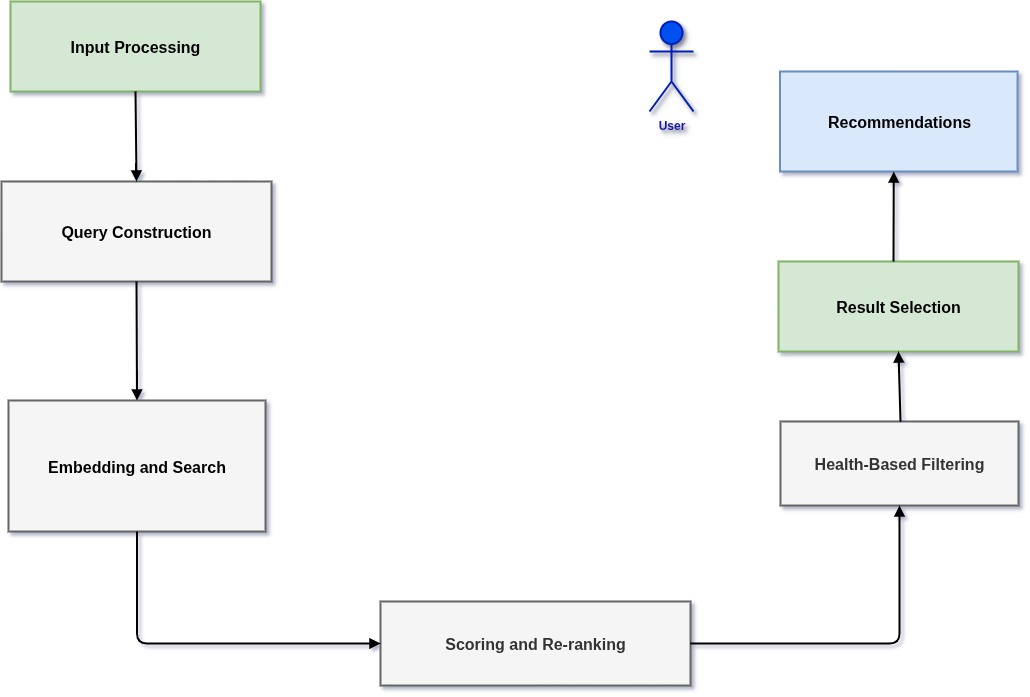
\includegraphics[width=0.9\textwidth]{images/CB_recommendation_workflow_simple.png}
\caption{Content-based recommendation workflow}
\label{fig:cb_workflow}
\end{figure}

\section{Collaborative Filtering Module}
\subsection{LightFM for Implicit Feedback}
LightFM implements matrix factorization optimized for implicit feedback (e.g., clicks, likes). It learns latent user and item embeddings to predict affinity.


\subsection{Interaction Matrix Design}
User actions are weighted to reflect preference strength:

\begin{table}[H]
\centering
\caption{Interaction types and weights}
\label{tab:interaction_weights}
\begin{tabular}{lcc}
\toprule
\textbf{Interaction} & \textbf{Weight} & \textbf{Interpretation} \\
\midrule
Liked & 1.0 & Strong positive \\
Visited & 0.5 & Mild interest \\
Disliked & -1.0 & Explicit negative \\
\bottomrule
\end{tabular}
\end{table}

\subsection{Loss Function Selection}
LightFM supports multiple loss functions:
\item \textbf{WARP}: Ignores negative feedback—unsuitable for our use case.
    \item \textbf{Logistic}: Requires explicit ratings—not applicable.
    \item \textbf{BPR (Bayesian Personalized Ranking)}: Optimizes pairwise ranking of liked vs. disliked/visited items.

We selected **BPR** to fully leverage explicit dislikes and ensure robust ranking.

\begin{figure}[H]
\centering
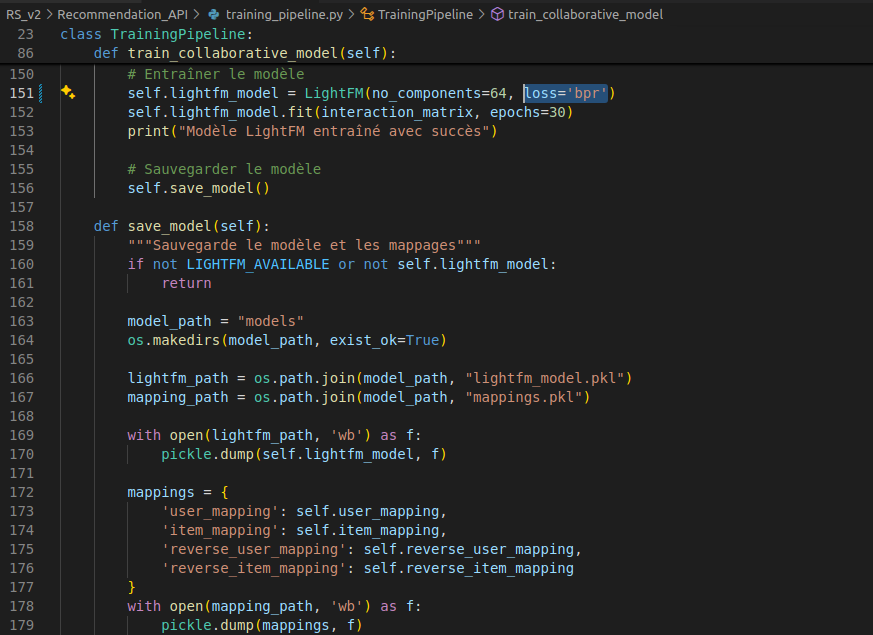
\includegraphics[scale=0.39]{images/loss_function_lightFM.png}
\caption{Training LightFM with BPR loss}
\label{fig:BPR_loss_function}
\end{figure}

\section{Scalability: Exact vs. Approximate Search}
\subsection{The Need for ANN in Production}
Exact cosine similarity search becomes infeasible beyond ~10K vectors. To ensure scalability, we benchmarked ChromaDB’s **HNSW-based ANN** against its default exact search.

\subsection{Theoretical Trade-offs}
\begin{table}[H]
\centering
\caption{Exact vs. HNSW search: key differences}
\label{tab:theoretical-comparison}
\resizebox{0.9\textwidth}{!}{%
\begin{tabular}{|l|c|c|}
\hline
\textbf{Feature} & \textbf{Exact Search} & \textbf{HNSW (ANN)} \\
\hline
Accuracy & 100\% & High (configurable) \\
Speed & Slow (O(n)) & Fast (sub-linear) \\
Memory & Low & Higher (graph index) \\
Scalability & <10K vectors & Millions of vectors \\
\hline
\end{tabular}
}
\end{table}

\subsection{Empirical Benchmark}
Tested on 23,000 products with 20,000 queries:

\begin{table}[H]
\centering
\caption{Performance benchmark}
\label{tab:benchmark-results}
\resizebox{0.7\textwidth}{!}{%
\begin{tabular}{|l|c|c|c|}
\hline
\textbf{Mode} & \textbf{Avg. Latency (ms)} & \textbf{Results/Query} & \textbf{Success Rate} \\
\hline
Exact & 187.4 & 10 & 100\% \\
HNSW & 178.08 & 10 & 100\% \\
\hline
\end{tabular}
}
\end{table}

HNSW delivers **5\% faster response times** with identical result quality at this scale—and will scale far better as the catalog grows. It is now the production default.

\section{Deployment and Integration}
\subsection{FastAPI Backend}
The system is exposed via a private FastAPI service with a single endpoint:
\begin{verbatim}
POST /recommend
\end{verbatim}
Input: \texttt{user\_id}, \texttt{ean} (optional), \texttt{limit}, \texttt{recommendation\_type}.

\begin{figure}[H]
\centering
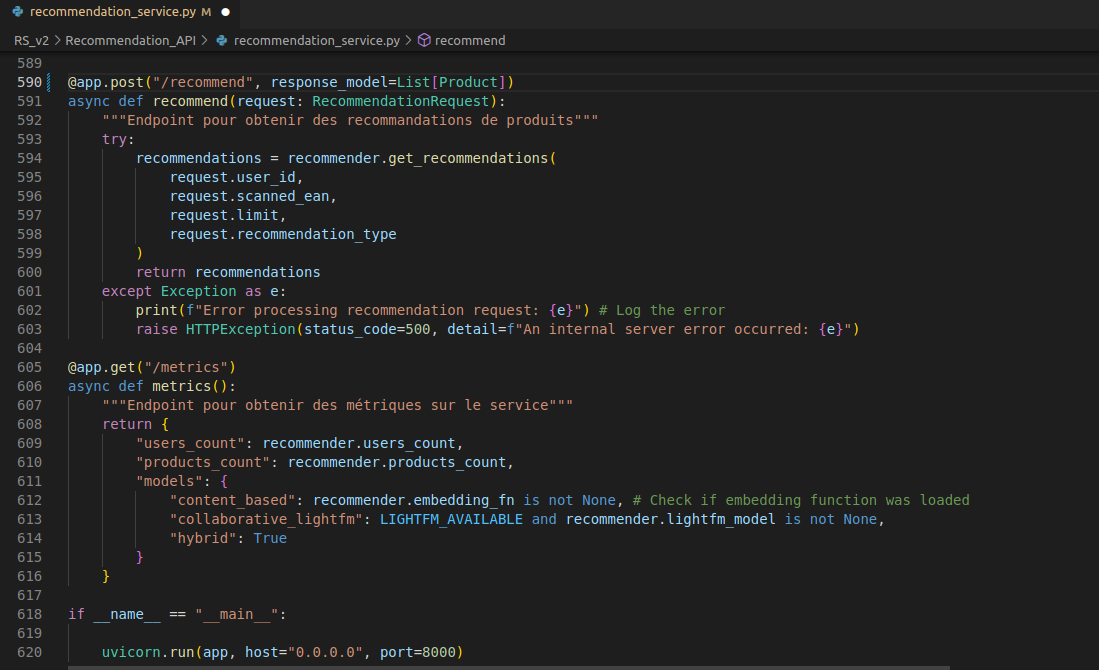
\includegraphics[scale=0.35]{images/deploy_RS.png}
\caption{Deployment architecture with FastAPI}
\label{fig:Deploy_RS}
\end{figure}

\subsection{Multi-Modal Recommendation Modes}
The \texttt{recommendation\_type} parameter supports:
\begin{enumerate}
    \item \texttt{"collaborative"} – LightFM only
    \item \texttt{"content"} – ChromaDB only
    \item \texttt{"hybrid"} – Weighted fusion (60/40)
\end{enumerate}

Internal access only (mobile app + dev team), with full documentation via Swagger UI.


\section*{Conclusion}
This chapter has outlined the architectural and algorithmic foundations
of the VitamiNurse recommendation system. The system employs a
modular, hybrid architecture that separates collaborative and contentbased filtering to achieve a balance between scalability and precision.
Integration of ChromaDB with HNSW indexing facilitates efficient semantic analysis of user needs and product attributes. Additionally, the
LightFM model, trained using a Bayesian Personalized Ranking (BPR)
loss function, effectively captures dynamic user preferences derived from
implicit feedback.
By concentrating on the user health condition, allergies and health goals,
the recommendation system suggests more healthy and personalized
products. However, providing effective guidance also requires an intuitive
and interactive tool. To address this need, the next chapter introduces
VitamiNurse AI assistant, designed to deliver real-time, conversational
support that bridges large language models with user-friendly interaction.


\chapter{Product Evaluation and AI Assistant in VitamiNurse}
\section*{Introduction}
\addcontentsline{toc}{section}{Introduction}
The VitamiNurse app stands out from other traditional nutrition apps through its advanced use of artificial intelligence .

In addition to the use of a sentence transformer model to generate vector embeddings in the recommendation system discussed earlier, this section introduces two key AI components: a product evaluation system and an AI assistant.

This integration of AI transforms static product recommendations into an interactive dialogue system that is available 24/7 to answer questions and provide nutritional guidance. The following sections detail the architecture and functionality of these AI systems within the VitamiNurse mobile app.

\section{Advanced scan system with AI analysis }

Instead of showing large amounts of raw product data, it uses AI to interpret the product after scanning its barcode.  Through the combination of detailed nutritional information, user health profiles, and AI reasoning based on prompts, the VitamiNurse app provides customized nutritional guidance in a way that traditional tools cannot. The result is a highly interactive and user-friendly experience that transforms a simple scan into an informed decision-making process.

\subsection{Prompt Engineering for AI Analysis}
\par In addition to the details of the product that appear on the screen after scanning the barcode, we added an AI analytics system to provide a concise and personalized conclusion.
 The generative AI capabilities of our system are powered by a popular pre-trained LLM, which is ChatGPT-4, to build accurate and relevant responses.
 \par The system uses structured prompts to guide AI during product evaluation.
The following code illustrates how each prompt integrates essential product information with user-specific data, including health conditions and allergies, to determine the suitability of the product for the user profile.
\begin{center}
\begin{figure}[H]
    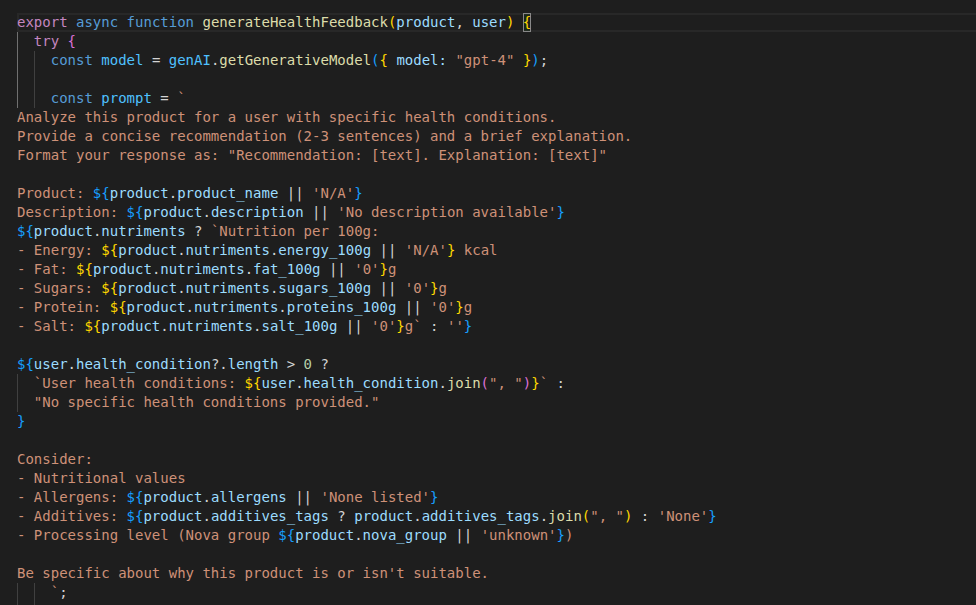
\includegraphics[width=0.9\textwidth]{images/prompt_engineering.png}
    \caption{Prompt Engineering Using GPT-4} 
    \label{fig:Prompt_Engineering}
\end{figure}
\end{center}

\subsection{System Operation in VitamiNurse}
The AI analysis system in VitamiNurse integrates a product scanning feature with real-time health feedback, powered by a combination of external APIs, a MongoDB database, and the ChatGPT-4 model. Users can scan a barcode (EAN) to retrieve detailed nutritional information, which is cross-referenced with their health profile stored in the users collection. The system first checks our database for existing product data. If it is unavailable, it fetches data from the OpenFoodFacts API and caches it for future use. The AI then processes these data alongside user health conditions to generate personalized feedback: \textbf{Is this product suitable or not, and why?}
The following picture illustrates how the user see the details of the scanned product and generated health feedback by the AI analytics system:
\begin{center}
    \begin{figure}[H]
    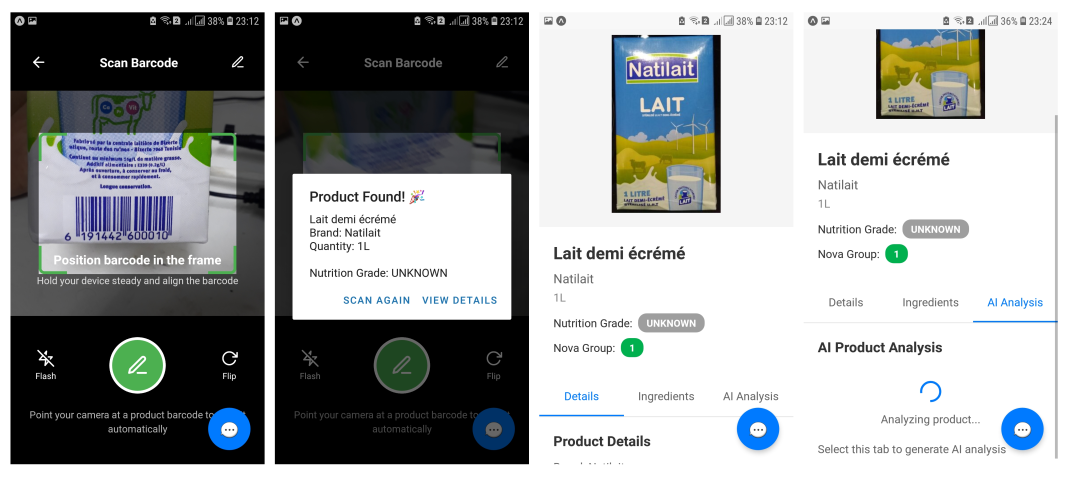
\includegraphics[width=0.9\textwidth]{images/natilait.png}
    \caption{Product evaluation and AI analysis in VitamiNurse app}
    \label{fig:main_figure}
\end{figure}
\end{center}

\section{The AI Assistant}
The AI nutrition assistant represents a new generation of personalized dietary advice and nutritional data analysis, all within a coherent conversational interface.
\section{System Architecture}
The architecture of the Nutrition Assistant is designed for modularity, scalability, and maintainability. Figure~\ref{fig:chatbot_Architect_layers} outlines this three-tier architecture, consisting of the user mobile interface, backend server, and AI/data layer.
 This separation ensures that improvements in one layer, such as up-grading the recommendation logic, can be implemented without disrupting other components of the system. The conversational capabilities of this intuitive chatbot are tightly integrated with a persistent memory framework in order to recall previous user interactions and adapt recommendations over time.  
\begin{figure}[H]
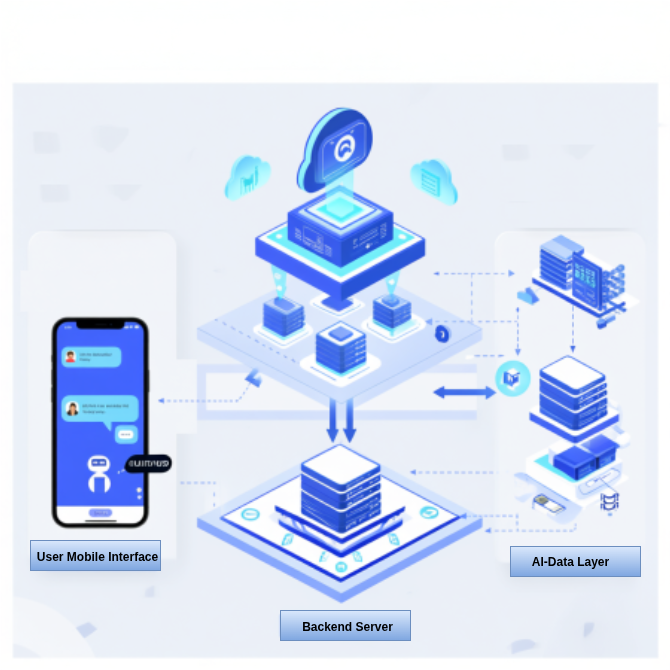
\includegraphics[width=0.9\textwidth]{images/chat_layers.png}
\caption{Chatbot Architecture} 
\label{fig:chatbot_Architect_layers}
\end{figure}

\subsection{User Mobile Interface}
The mobile interface functions as the central interaction point for users
engaging with the VitamiNurse assistant, supporting key features such
as conversational dialogue and product scanning. When a user scans a
product barcode or types a question, the interface sends a structured
request to the backend, which in turn invokes the AI modules for analysis.
The design emphasizes simplicity and readability, ensuring that even
complex nutritional assessments are communicated in concise and easy-to-understand language. 
This is achieved through the adoption of a fixed
“Recommendation + Explanation” format, which the AI adheres to
when generating responses. The application returns the scanned product’s details and nutritional breakdowns as well as AI analysis for this product,
making the experience both informative and engaging.

\begin{center}
\begin{figure}[H]
\centering
\includegraphics[width=0.51\textwidth]{images/chat_interface.jpg}
\caption{AI assistant chat interface} 
\label{fig:chatbot_interface}
\end{figure}
\end{center}


\subsection{Backend (FastAPI Server)}
The backend, developed using the \textbf{FastAPI} framework, functions as the system’s control hub. It is responsible for orchestrating communication between the mobile interface, AI reasoning layer, and data storage modules. Upon receiving a request, the backend validates the input, retrieves relevant product data from the nutritional database, and enriches it with user-specific profile information. It then constructs a prompt to be sent to the large language model (LLM), ensuring that all relevant dietary constraints and health conditions are explicitly included. The backend also maintains user session management, conversation history storage, and security protocols for handling sensitive health-related information. Thanks to FastAPI’s asynchronous capabilities, the backend can handle concurrent user requests with minimal latency, which is crucial for providing real-time responses.
\begin{center}
\begin{figure}[H]
\includegraphics[width=0.9\textwidth]{images/chatbot_API.png}
\caption{Chatbot FastAPI} 
\label{fig:chatbot API}
\end{figure}
\end{center}

\subsection{AI and Data Layer}
The AI and data layer forms the intelligent core of the VitamiNurse assistant, leveraging advanced language models and sophisticated intent detection to deliver personalized nutritional guidance. At the heart of the system is OpenAI's \texttt{gpt-4o-mini} model, which is meticulously engineered through prompt crafting to provide structured, scientifically-grounded nutritional advice.

The system employs \texttt{LangChain} as its orchestration framework, enabling sophisticated intent detection and parallel processing of user requests. Through LangChain's structured output parsing with Pydantic models, the assistant can simultaneously handle multiple user intents including product searches, recipe generation, profile updates, and general nutritional inquiries.

A \texttt{ChromaDB} vector database serves as the persistent storage layer, maintaining semantic embeddings of user profiles, conversation history, and product information. This enables efficient retrieval and contextual understanding while ensuring data persistence across sessions.

The \emph{Recommendation Engine} introduced in the previous chapter is seamlessly integrated into this architecture. It operates on a hybrid approach combining collaborative filtering and content-based filtering, ensuring that recommended products are both personalized and nutritionally appropriate for each user's specific profile and constraints.


\section{Retrieval-Augmented Generation (RAG) in VitamiNurse}
\label{sec:rag}

\par Retrieval-Augmented Generation (RAG) is a hybrid architecture that enhances large language model (LLM) responses by dynamically retrieving relevant external knowledge and integrating it into the generation process \cite{lewis2020retrieval}. In the context of the \textit{VitamiNurse AI Assistant}, RAG enables personalized, context-aware nutritional guidance by retrieving user-specific health profiles and interaction history from a persistent vector database before generating responses. This approach ensures that advice is not only linguistically fluent but also grounded in the user’s unique physiological and dietary context. Formally, RAG decomposes into three sequential stages: Retrieval (R), Augmentation (A), and Generation (G) as illustrated in Figure~\ref{fig:RAG_architecture}

\begin{center}
\begin{figure}[H]
\includegraphics[width=0.98\textwidth]{images/RAG_logic.png}
\caption{RAG architecture in VitamiNurse} 
\label{fig:RAG_architecture}
\end{figure}
\end{center}

\subsection{Retrieval (R): User-Centric Context Fetching}
\label{subsec:retrieval}

The retrieval phase in VitamiNurse leverages \texttt{ChromaDB} to fetch semantically relevant user information. Specifically, two collections are maintained:
\begin{itemize}[label=-]
\item users : Stores structured user profiles (age, allergies, health conditions) as metadata, with embeddings generated via the \texttt{all-MiniLM-L6-v2} sentence transformer.
\item chat\_sessions : Archives past interactions to support short-term conversational memory.
\end{itemize}


When a user sends a message, the system retrieves their profile using their \texttt{user\_id}. This exact-match retrieval (by ID) is complemented by semantic capabilities for future extensions (e.g., similarity-based health cohort lookup). The retrieved profile serves as the primary source of personalization, aligning with RAG’s principle of grounding generation in external knowledge\cite{rag2020}.

\subsection{Augmentation (A): Dynamic Prompt Personalization}
\label{subsec:augmentation}

The augmentation phase constructs a system prompt that embeds the retrieved user profile into the LLM’s context window. VitamiNurse implements this via the \texttt{\_create\_personalized\_system\_prompt()} method, which formats user attributes (e.g., allergies, dietary preferences, pregnancy status) into natural language directives. For example:

\begin{quote}
    ``You are VitamiNurse, a nutrition AI. The user is a 32-year-old pregnant woman with celiac disease and a preference for high-fiber foods. Avoid gluten and prioritize iron-rich, pregnancy-safe options.''
\end{quote}

This step ensures the LLM’s internal reasoning is conditioned on factual, user-specific constraints—reducing hallucination risks and improving relevance. The augmented prompt, combined with recent conversation history (up to 6 turns), forms the complete input to the generator.

\subsection{Generation (G): Personalized Response Synthesis}
\label{subsec:generation}

The generation phase employs \texttt{gpt-4o-mini} model from OpenAI to produce concise and informed responses with specific instructions to limit replies to three sentences for clarity. In order to maintaining focus within the application’s intended scope ,the model is designed to gently but firmly redirect the discussion back to nutrition-related subjects.

\begin{quote}
    ``I can only provide nutritional advice. For medical concerns, please consult a healthcare professional.''
\end{quote}
Critically, generation it is \textit{conditioned} on the augmented prompt from the augmentation phase . After the response is sent, the conversation is saved in the background to the \textbf{chat sessions} database, and this closes the RAG loop by enabling future use of the interaction.

Additionally, the system uses the LLM itself to extract and update profile information from user messages such as detecting new allergies, effectively using generation to enrich the knowledge base this feature known as \textit{write-path RAG} }. In this case, the RAG system does not only retrieve and generate as in the traditional read-path process, but also updates or writes new information back into the user collection in ChromaDB based on chat interactions.

\section{Challenges and Solutions}
Throughout development, several significant challenges emerged in creating a robust conversational nutrition assistant. Maintaining coherent conversation context across extended interactions was addressed through LangChain's sophisticated memory management and ChromaDB's persistent conversation storage. Personalizing recommendations without burdening users with excessive input requirements was solved through GPT-4's intelligent information extraction capabilities, which automatically detect and update user profiles from natural conversation.

Ensuring structured, explainable nutritional advice was achieved through rigorous prompt engineering and Pydantic output parsing, enforcing consistent response formats. Handling ambiguous or incomplete user queries was resolved through the parallel intent processing architecture, which allows multiple interpretation paths to be explored simultaneously before synthesizing a comprehensive response.

The integration of multiple AI components (LangChain chains, GPT-4, ChromaDB, and the recommendation API) presented coordination challenges that were overcome through asynchronous processing patterns and robust error handling mechanisms.

\section{Future Improvements}
Planned enhancements focus on expanding the assistant's capabilities and integration points. Multi-modal support will enable image-based food recognition and nutritional analysis through advanced computer vision integration. Expanded wearable device connectivity will incorporate real-time physiological data from fitness trackers and health monitors, allowing for dynamic nutritional adjustments based on activity levels and metabolic states.

Advanced personalization through reinforcement learning will enable the system to continuously improve its recommendations based on user feedback and outcomes. Voice interaction capabilities will be enhanced through integration with popular voice assistants (Alexa, Google Assistant) and development of custom voice interfaces for hands-free nutritional guidance.

Additional planned features include:
\begin{itemize}
\item \textbf{Meal Planning Automation}: Multi-day meal planning with grocery list generation
\item \textbf{Social Features}: Community recipe sharing and nutritional challenges
\item \textbf{Healthcare Integration}: EHR connectivity for medical condition management
\item \textbf{Advanced Analytics}: Nutritional intake tracking and trend analysis
\end{itemize}


\section{Conclusion}
The VitamiNurse AI Nutrition Assistant represents a significant advancement in conversational healthcare applications by successfully integrating the Recommendation Engine into a sophisticated LangChain-powered architecture. The system demonstrates how parallel intent processing, dynamic profile management, and AI-generated content can create a comprehensive nutritional guidance platform.

By leveraging LangChain's orchestration capabilities alongside GPT-4's generative power and ChromaDB's persistent storage, VitamiNurse delivers personalized, context-aware dietary recommendations that adapt to users' evolving needs. The architecture successfully balances conversational flexibility with structured nutritional guidance, providing both immediate answers and long-term nutritional support.

This implementation positions VitamiNurse as a scalable foundation for digital health interventions, with the potential to expand into various healthcare domains beyond nutrition. The modular design ensures adaptability to new data sources, interaction modalities, and user requirements, making it well-suited for the evolving landscape of AI-powered healthcare applications.

The assistant not only provides immediate nutritional guidance but also serves as an educational tool, helping users develop sustainable healthy eating habits through personalized, explainable recommendations that consider their unique circumstances, preferences, and goals.


\chapter*{General Conclusion}
\addcontentsline{toc}{section}{General Conclusion}
The VitamiNurse project represents a significant step forward in the integration of artificial intelligence into personalized nutrition and digital health. 
By combining a robust data pipeline, 
a hybrid recommendation system, and an intelligent conversational assistant, this work delivers a holistic solution that addresses key limitations observed 
in existing nutritional applications, the lack of personalization, real-time adaptability, interactivity, and contextual awareness. 

Throughout this internship at ONRTECH, we successfully designed and implemented several core components that collectively transform VitamiNurse from a basic 
barcode scanner into an intelligent nutritional companion. The Nutri-pred-v1 model ensures data completeness by accurately predicting missing nutritional values, 
thereby enhancing the reliability of downstream analyses. The ETL pipeline enables continuous ingestion and enrichment of product data from diverse European sources, 
while standardization and multilingual handling ensure global applicability. 

The hybrid recommendation system that we developed combines both collaborative filtering via LightFM and semantic content-based retrieval to deliver highly personalized suggestions tailored to each user’s dietary restrictions and medical conditions. 
Benchmarking confirmed that the use of HNSW-based approximate nearest neighbor search provides an optimal balance between speed and accuracy and  ensures scalability for real-world deployment. 
The architecture successfully balances conversational flexibility with structured nutritional guidance, providing both immediate answers and long-term nutritional support.

As a result, this implementation positions VitamiNurse as a scalable foundation for digital health interventions, with the potential to expand into various healthcare domains beyond nutrition. 
The modular design ensures adaptability to new data sources, interaction modalities, and user requirements, making it well-suited for the evolving landscape of AI-powered healthcare applications.

In conclusion, the VitamiNurse project demonstrates the transformative potential of AI in enhancing personalized nutrition and digital health. By leveraging advanced machine learning techniques and a user-centric design approach, we have created a solution that not only meets the immediate needs of users but also lays the groundwork for future innovations in the field.

% Bibliographie
\bibliographystyle{IEEEtran}
\bibliography{references}

\end{document}
